%%%%%%%%%%%%%%%%%%%%%%%%%%%%%%
% 	   美赛模板,正文部分		 
%          PAPER.tex         
%%%%%%%%%%%%%%%%%%%%%%%%%%%%%%

\documentclass[12pt]{article}

% 请在此填写控制号、题号和标题,年份不需要填(自动以当前电脑时间年份为准)
\usepackage[1916056]{easymcm}\problem{C}   
\usepackage{palatino} % 这个是COMAP官方杂志采用的字体,如不需要可注释掉,以使用默认字体
\title{xxx}  % 标题


% 如您参加的是ICM(即选择了D/E/F题),请使用以下的命令修改Summary Sheet题头
% \renewcommand{\contest}{Interdisciplinary Contest in Modeling (ICM) Summary Sheet}

% 正文开始
\begin{document}

\input{ABSTRACT.tex}		% 摘要请到ABSTRACT.tex中填写


%=============================== Introduction ==========================
\section{Introduction}
The United States is now experiencing an opioid crisis. In 1996, when the Pain Society called pain "the fifth vital sign", an increasing emphasis on managing American patient's pain emerged. Opioid, highly effective analgesic drugs, became a source of abuse used by addicts who could easily obtain and abuse the drug to achieve a quick high. According to the New York Times' comprehensive data from the states, the number of opioid overkills in 2016 may exceed 59000, resulting in economic losses of about \$78.5 billion. It's an urgent task for the United States to deal with an epidemic of opioid use. Our target is to investigate the spread and characteristics of opioid and try to find out related solutions.

In part I, we compared our problem with the idea of Susceptible-Infective-Susceptible (SIS) Epidemic model to describe the characteristics of the reported synthetic opioid and heroin incidents (cases) in the five states. Considering the spread is not independent ,we added external impact factor to predict the spread between five states.In part II, based on prediction of our model in part I and the U.S. Census socio-economic data provided, we use Analytic Hierarchy Process (AHP) to find the cause, trends and impact of opioid crisis. In part III, we identified a possible strategy for countering the opioid crisis, and used our models to test the effectiveness of this strategy.


%========================= Preprocessing of data ======================
\section{Preprocessing of data}
At first, we made a preprocessing of the NFLIS data. This process includes data screening and reorganization to show the spread and characteristics of the reported synthetic opioid and heroin incidents in and between the five states and their counties over time.
\begin{figure}[!htbp]
\small
\centering
\includegraphics[width=7cm]{Fig/2010_heroin.png}
\includegraphics[width=7cm]{Fig/2017_heroin.png}
\caption{Distribution of heroin among states in 2010 and 2017}
\end{figure}

\begin{figure}[!htbp]
\small
\centering
\includegraphics[width=7.3cm]{Fig/2010_others.png}
\includegraphics[width=7cm]{Fig/2017_others.png}
\caption{Distribution of other synthetic opioids among states in 2010 and 2017}
\end{figure}

Our team has plotted the figures from 2010 to 2017. Due to the page limit,we just select figures of heroin and synthetic opioids distribution in 2010 and 2017, respectively, which serve as a comparison chart showing the trend change. The four figures above use areas of the circles to show the number of heroin and synthetic opioids samples in five states. The lager the area, the larger the number of samples, and vice versa. The pair of figures in orange (Fig.1) corresponds to the distribution of heroin, while the pair of figures in blue (Fig.2) corresponds to the distribution of other synthetic opioids.

The series of related figures help us more intuitively analyze trends with heroin and synthetic opioids in each state. It is obvious that the changes in each state are not monotonous, so we have supposed that the state's drug report has growth rates and reduction rates, which are for different objects.



\begin{figure}[!htbp]
\small
\centering
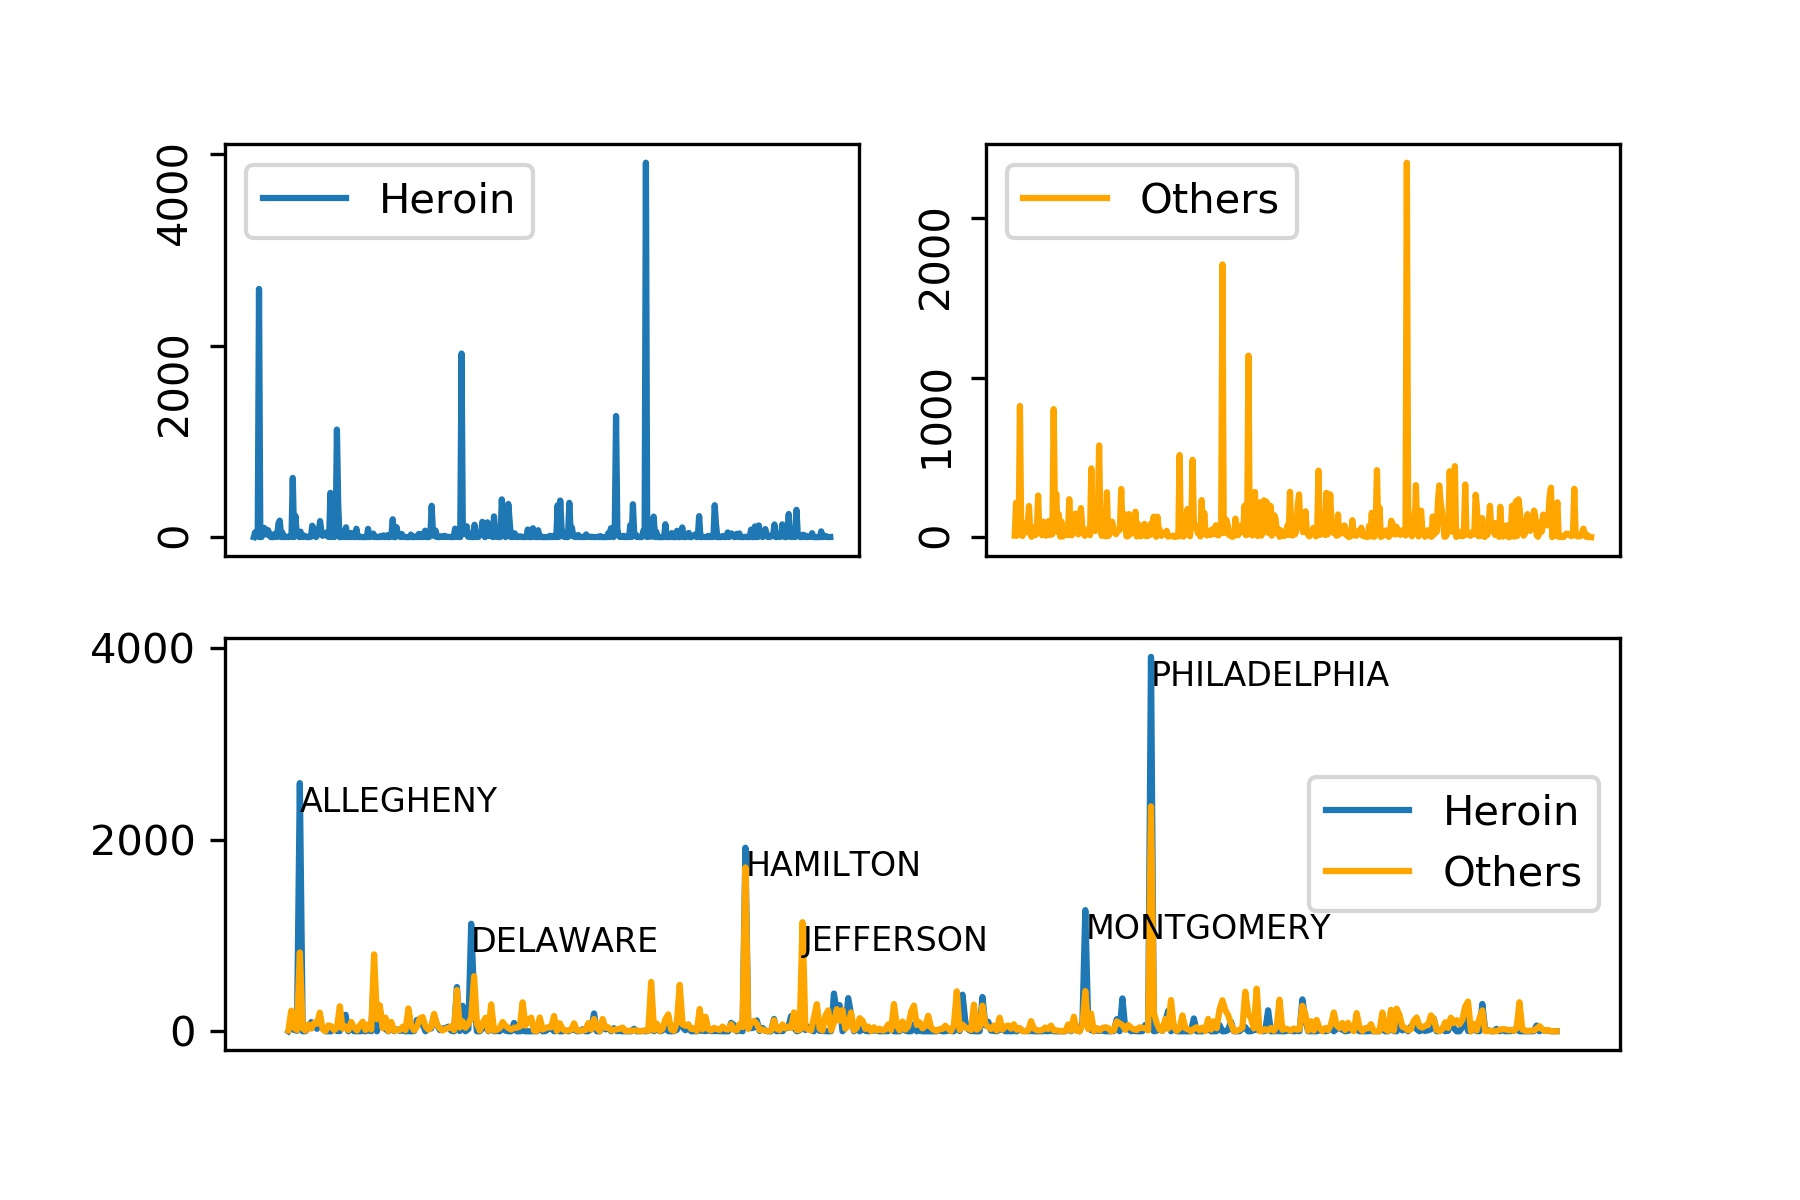
\includegraphics[width=12cm]{Fig/2010_Heroin_and_others(county).jpeg}
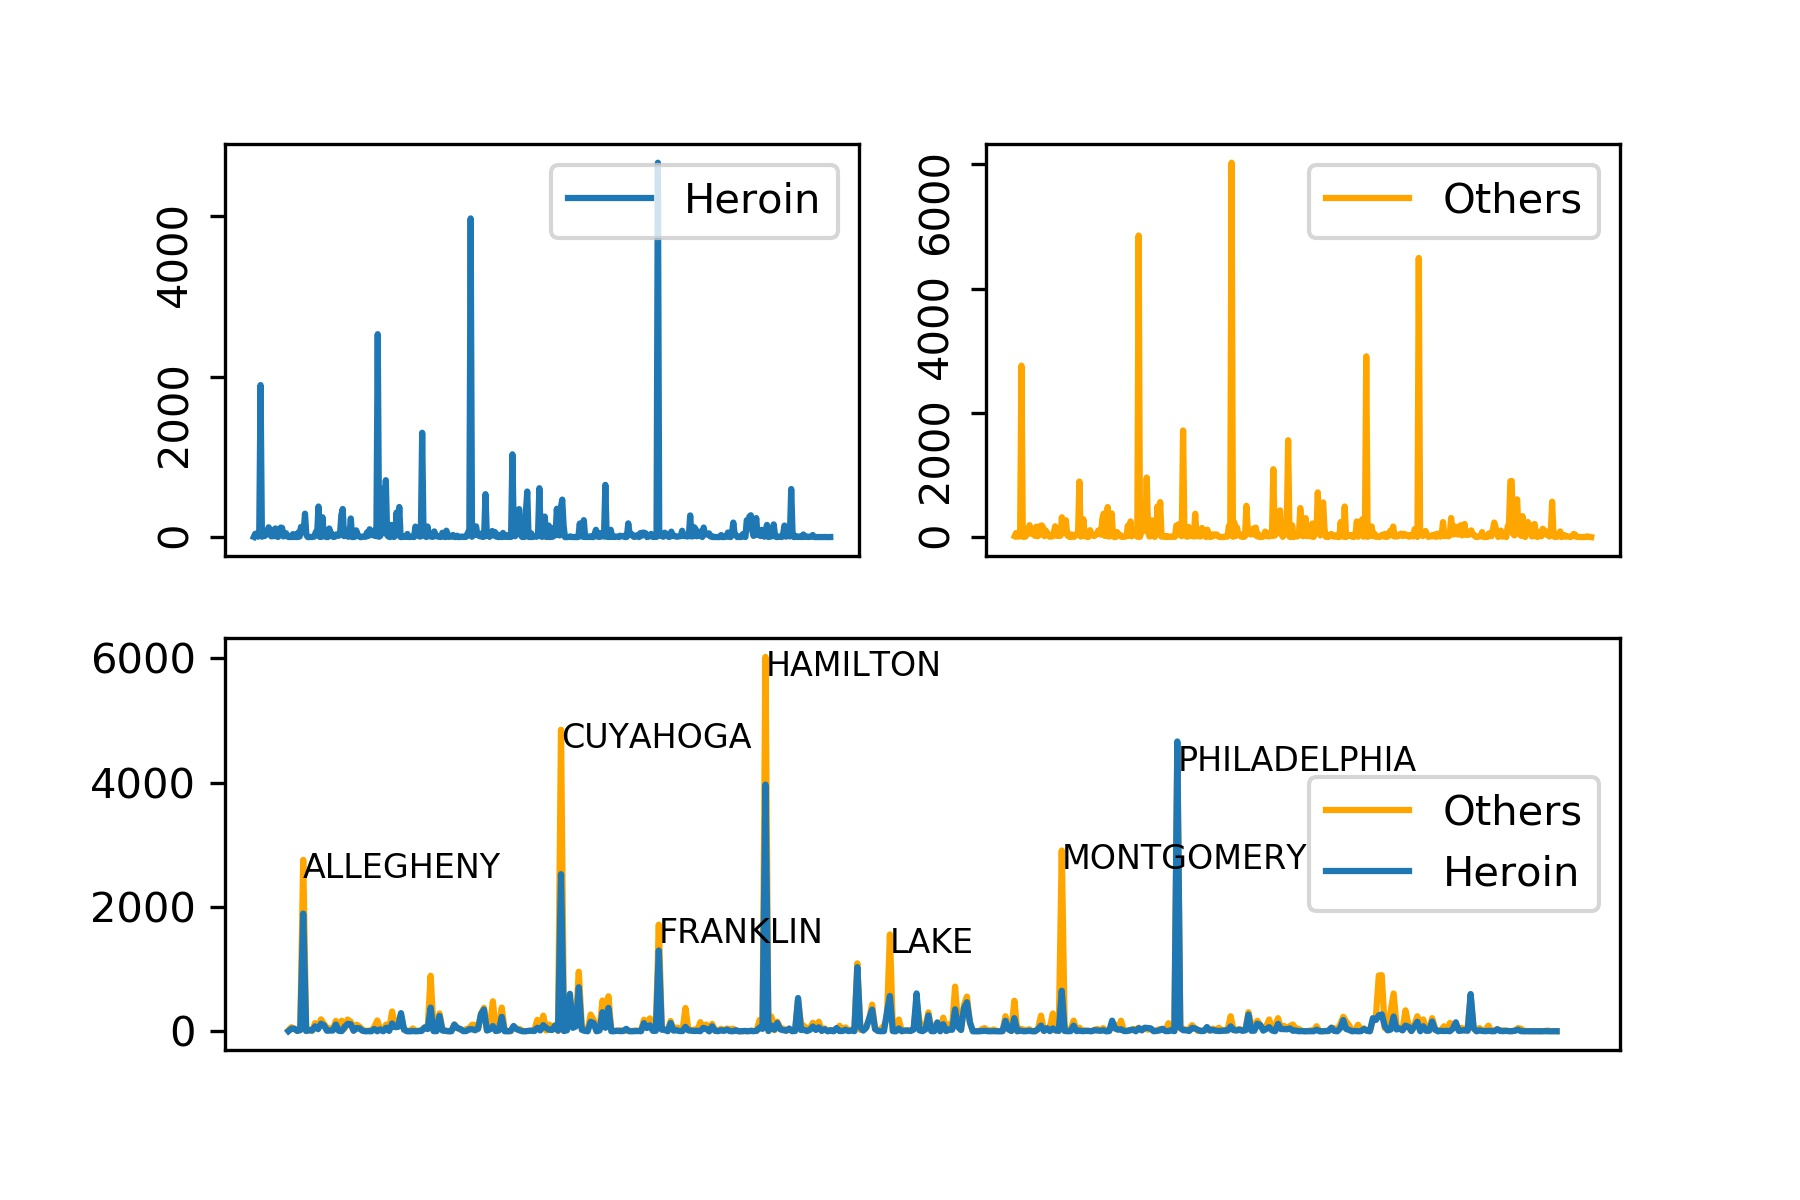
\includegraphics[width=12cm]{Fig/2017_Heroin_and_others(county).jpeg}
\caption{Distribution of heroin and other synthetic opioids among counties in 2010 and 2017}
\end{figure}

Fig.3 show the number of heroin and synthetic opioids distribution for different counties in 2010 (Fig.3[upper]) and 2017 (Fig.3[lower]).The X-axis represents different counties, and the Y-axis represents the number of drug reports in each county. We can find the counties with more drug reports than other counties, which is good for next analysis.  Also, We have synthesized two figures and found that high heroin reports are usually accompanied by high other drug reports.


\begin{figure}[!htbp]
\small
\centering
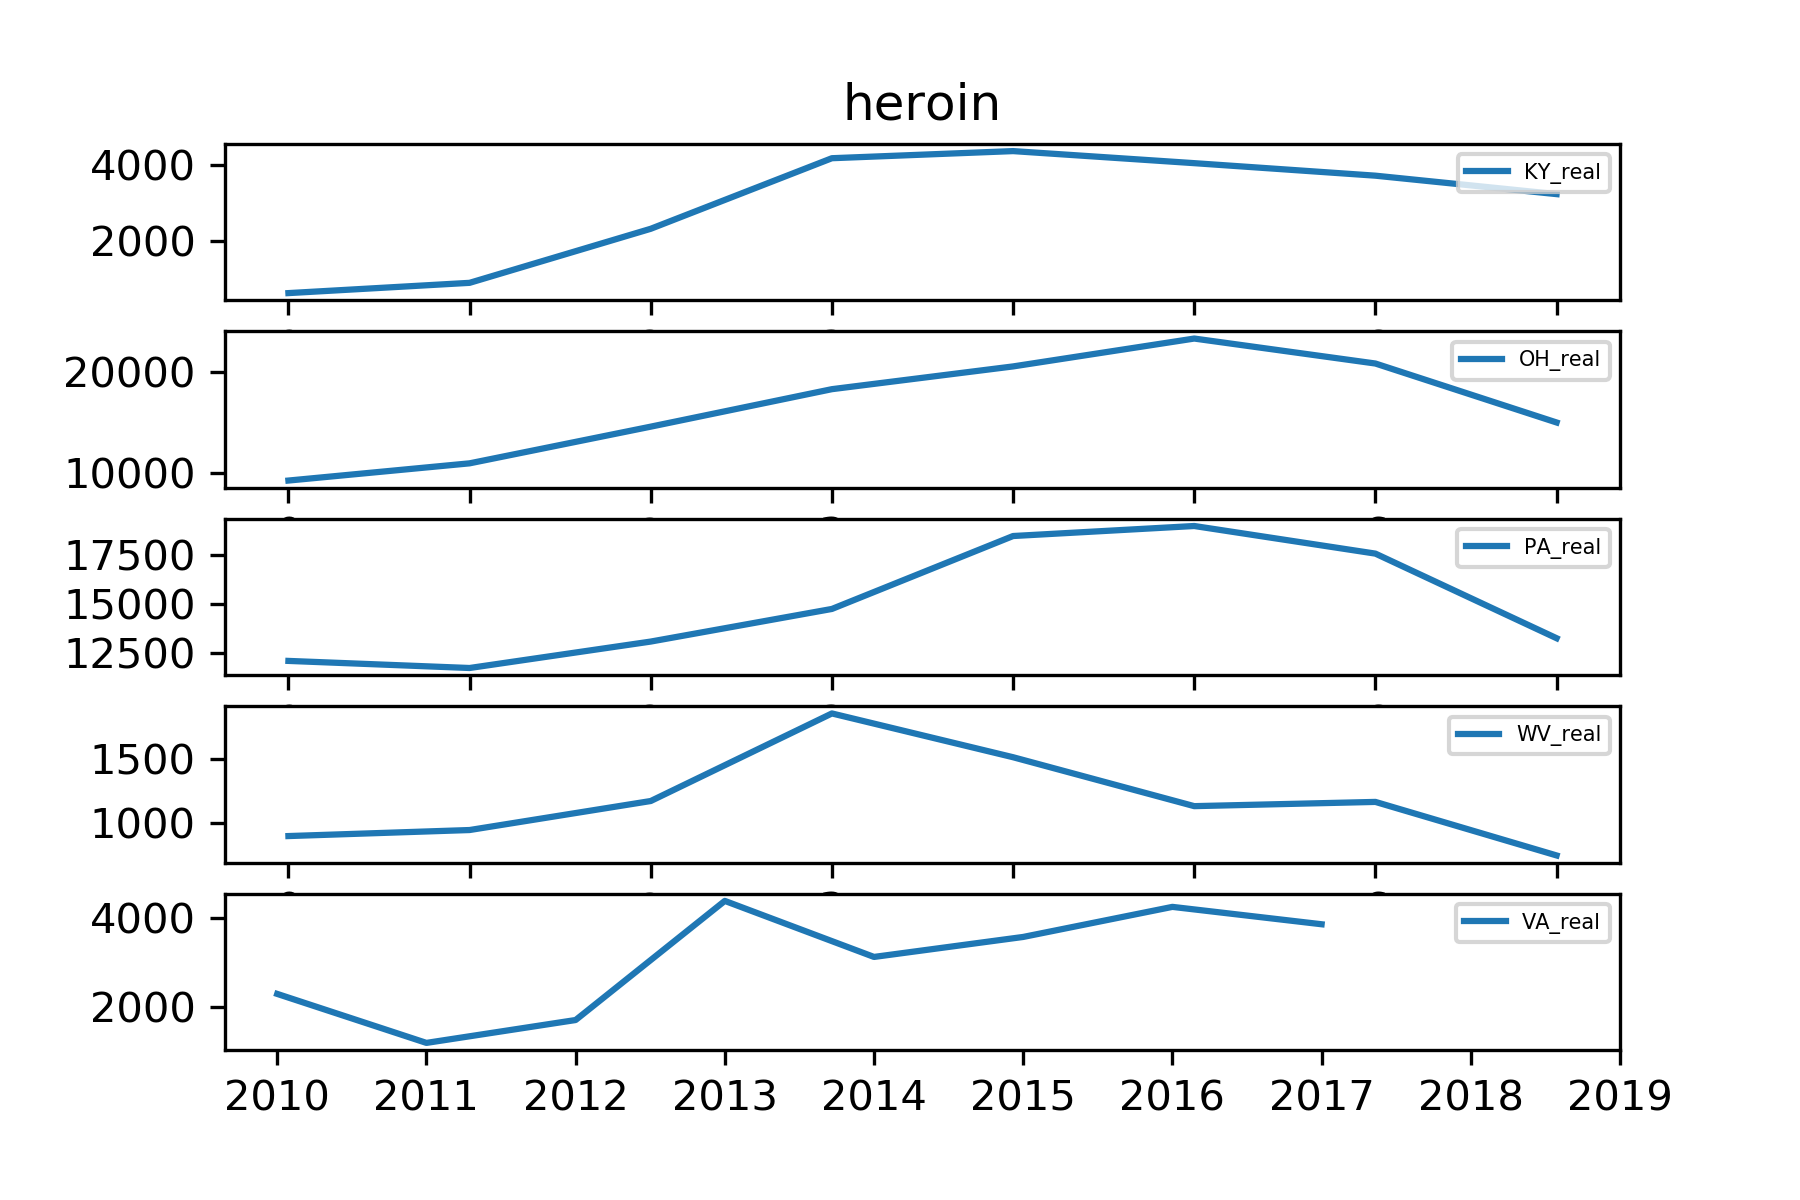
\includegraphics[width=14cm]{Fig/heroin_states_real}
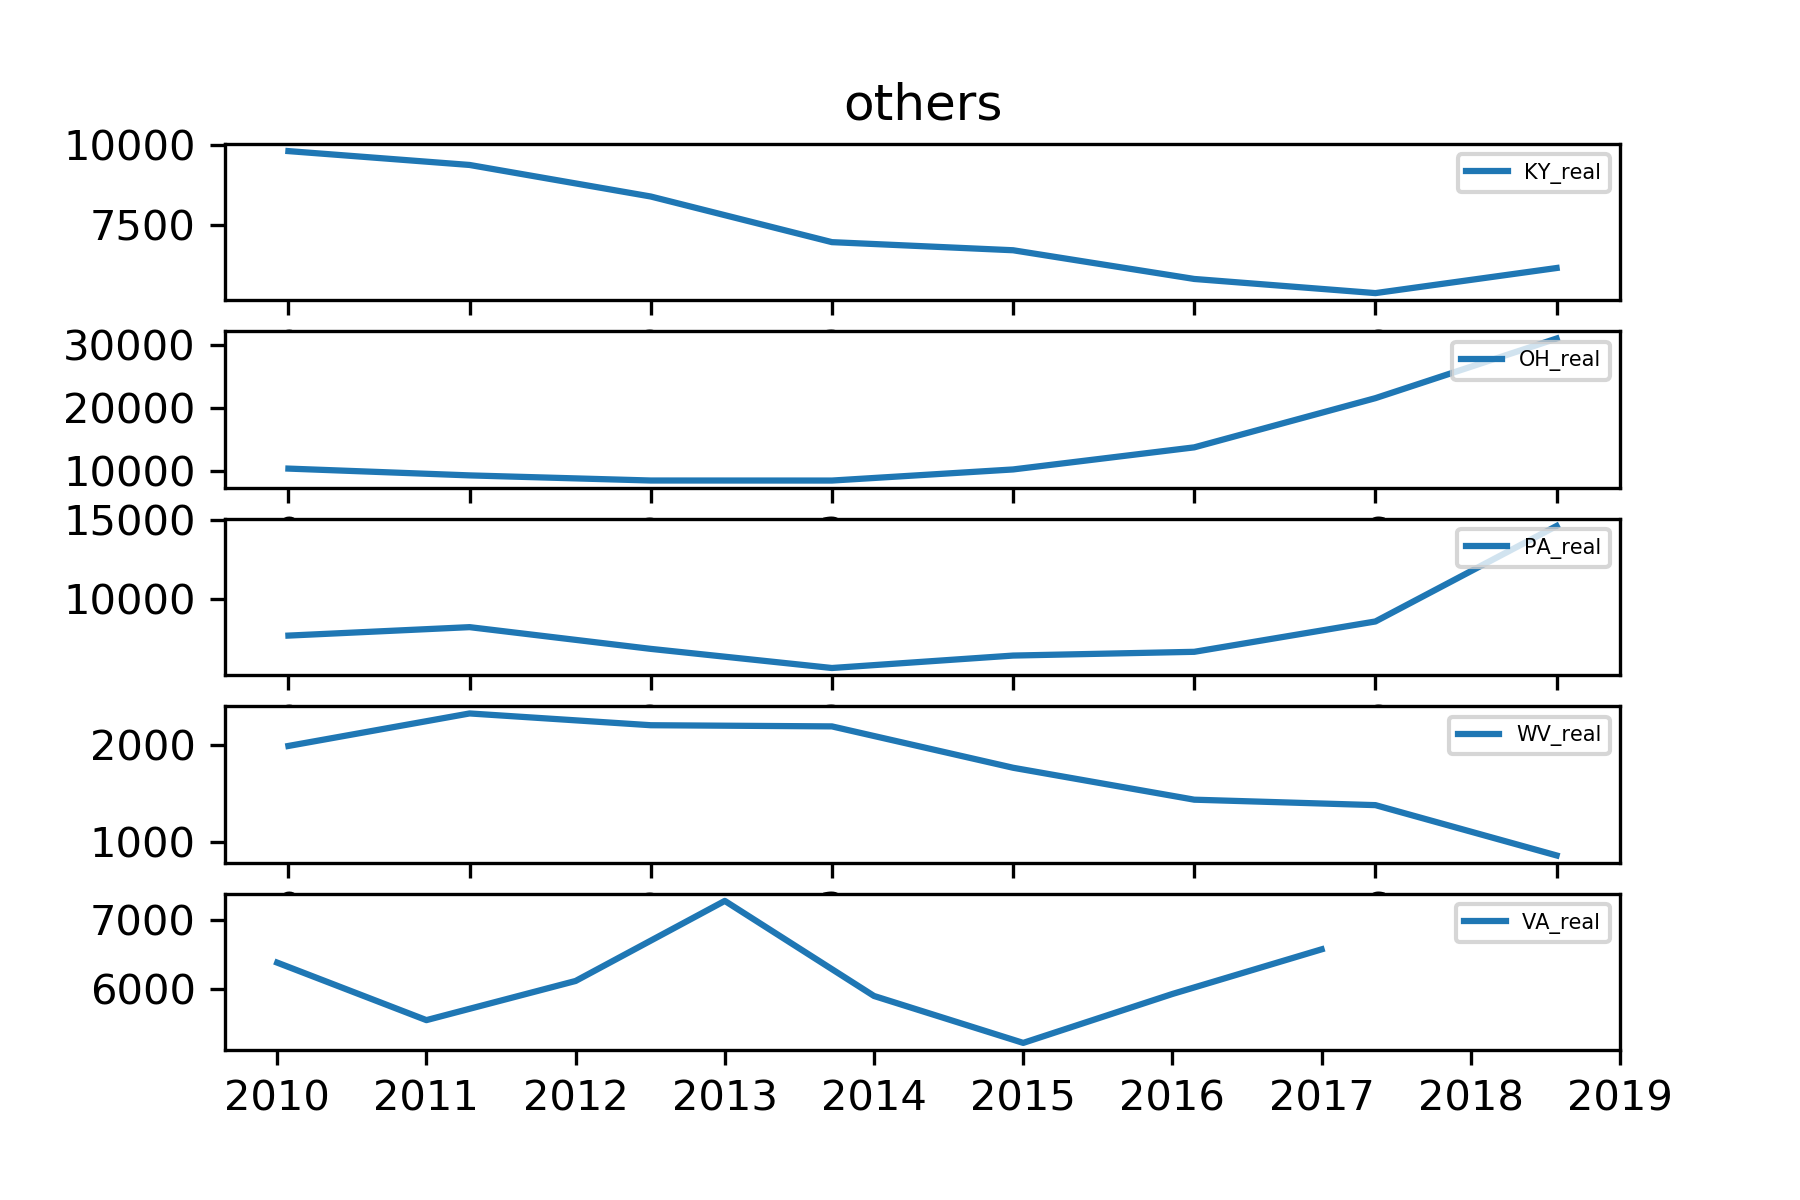
\includegraphics[width=14cm]{Fig/others_states_real}
\caption{Distribution of other synthetic opioids among states in 2010 and 2017}
\end{figure}

For a certain state in each year, we collect all the reports of Heroin and other substances and take the sums, respectively. As illustrated in Fig.4[upper], the total number of heroin in each state basically increases, reaches its peak sometime between 2015 and 2016 and then drops gradually after that (probably due to the interference from government). As for other substances shown in Fig.4[lower], we can see the trend similar to the spread of heroin over time in Fig.4[upper] (no matter it is increasing or decreasing, the change rate of slope is similar). Note that the curve of $VA$ in both Fig.4[upper] and Fig.4[lower] shows poor regularity, it may be treated as an outlier from which the majority of error of our model would derive.


%========================= Prelimiinary modle ======================
\section{Preliminary model}
\subsection{Notations}
Refer to Fig.5
\begin{figure}[!htbp]
\centering
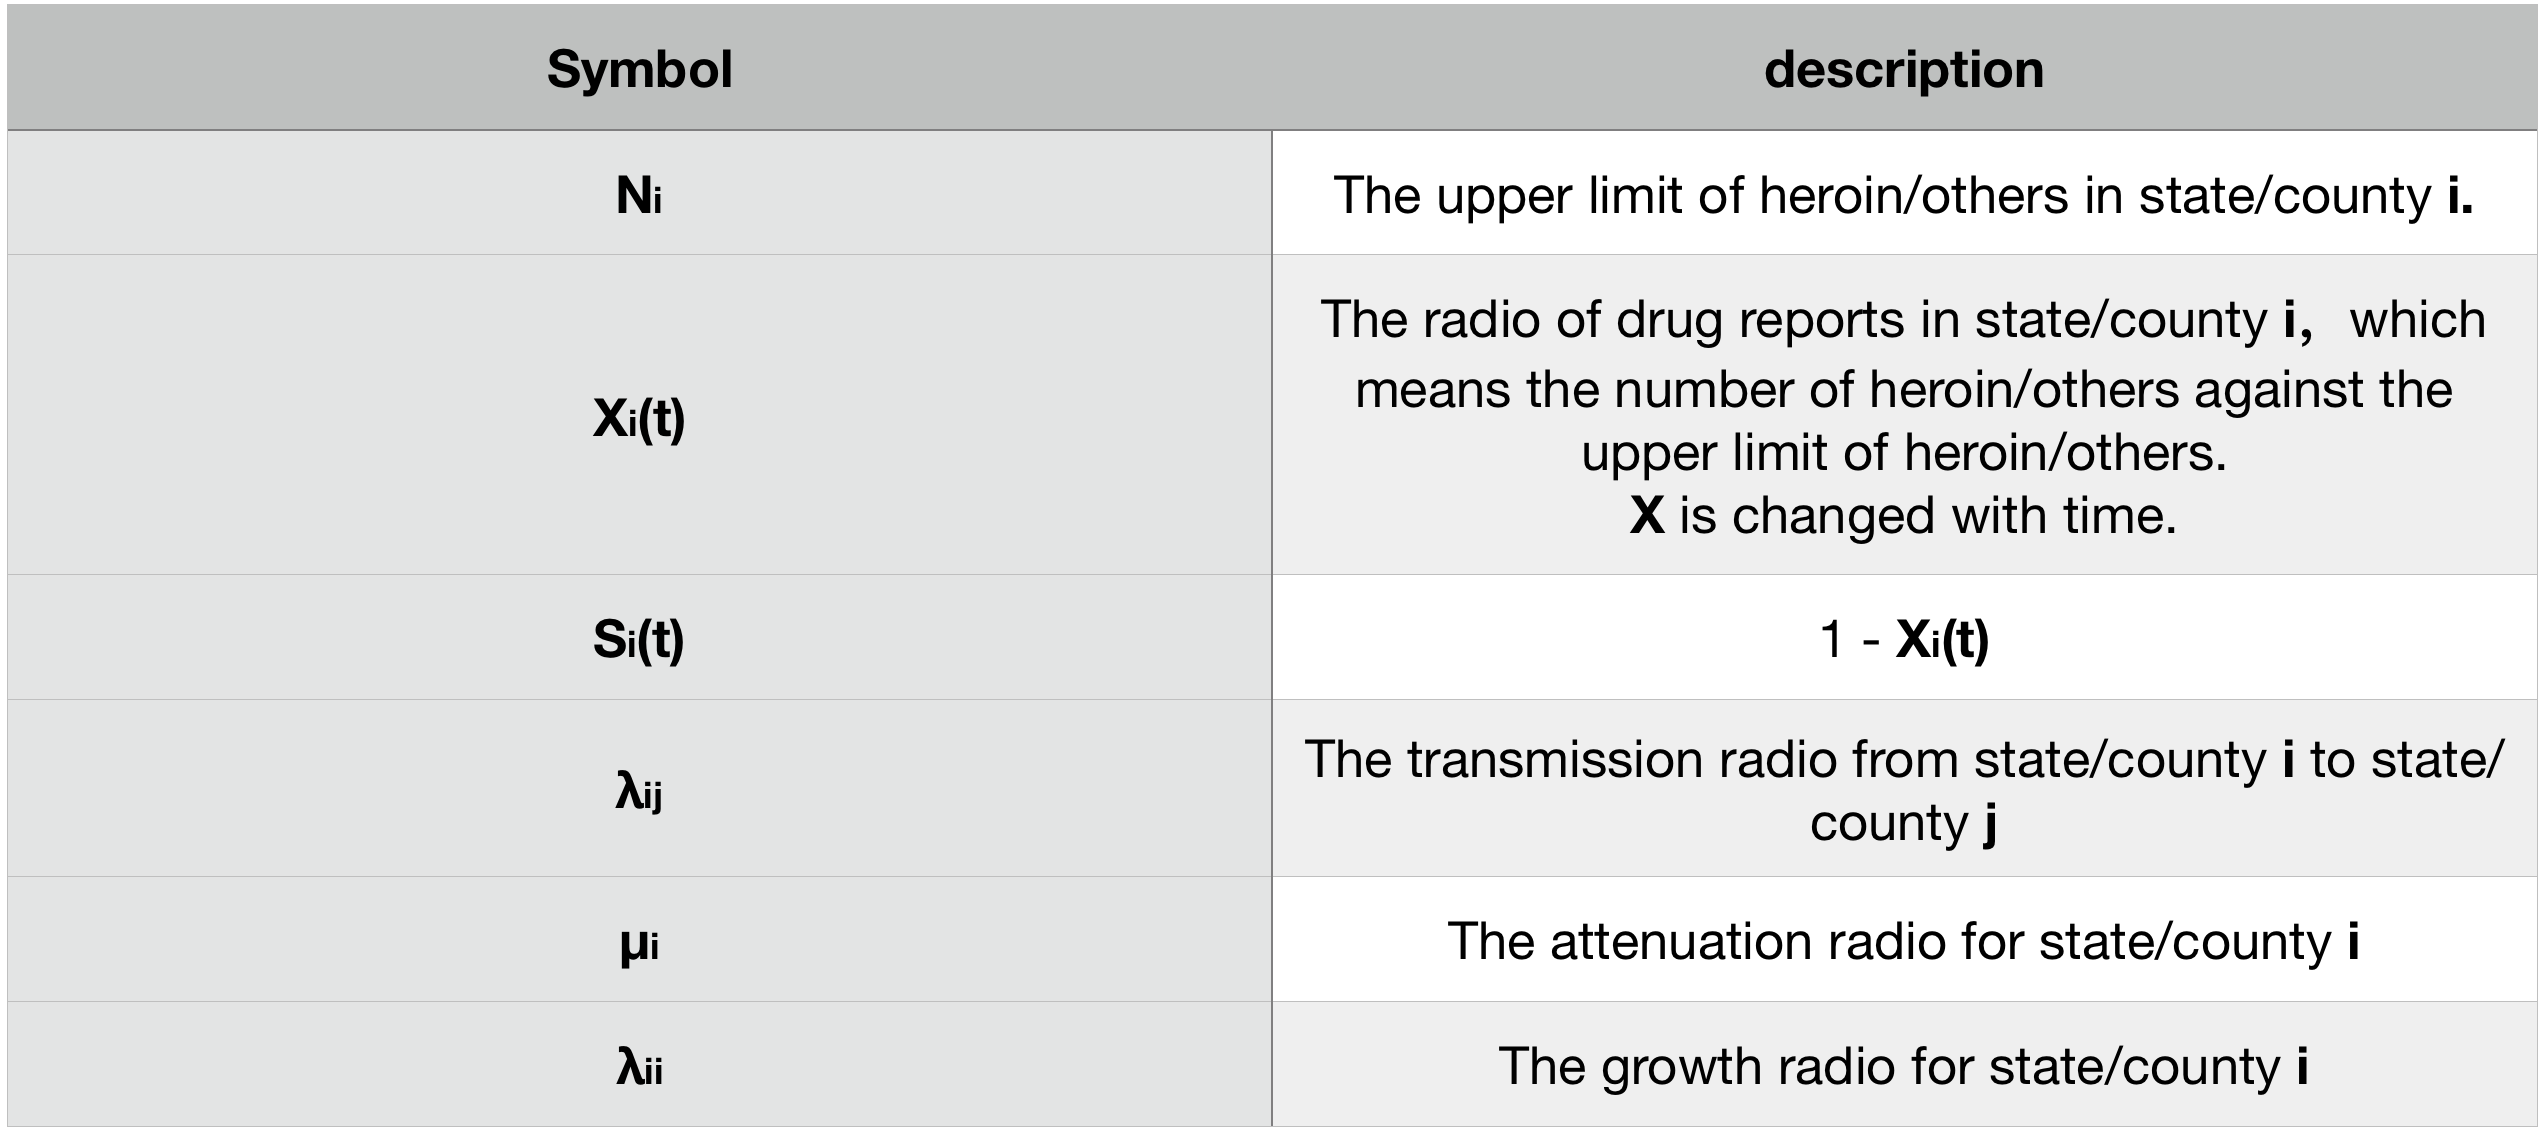
\includegraphics[width=16cm]{Fig/notations}
\caption{Symbol descriptions}
\end{figure}

\subsection{Assumptions}

\begin{enumerate}[\bfseries 1.]
    \item Opioids can be categorized into two groups: synthetic opioid and heroin (Four of every five heroin users start by misusing prescription painkillers, so heroin is a relatively different part of the opioids.)

    \item Changes in the number of opioids use are only affected by internal diffusion and external propagation.

    \item The amount of drug in every state has an upper limit. In other words, the spreading scope of drug is limited within the certain location for the simplification of our discussion

    \item The total amount of population is hypothetically divided into two groups, drug users and potential drug users.
    
    \item The growth rate of the drug $\lambda$ in every state is categorized into internal spreading and external introduction. The difference between the potential upper limit and the current number of drug is potential increment of one kind of certain drug.
    
    \item The consumption number of drugs in every state has its own rate of change $\mu$.
    
    \item The decay number of drugs is classified as the spreading yet to disseminate.
    
    \item Assuming that the number of a certain drug varies continuously with time.
\end{enumerate}

\subsection{Modeling}
\subsubsection{Basic model}
We used the SIS Epidemic model$^{[2]}$, assuming that the threshold for all opioid testing cases in each state (or county) is $N$. The radio of opioid reports in state (or county), which means the number of heroin (or others) over the upper limit of heroin (or others), is $x(t)$, and the radio of undetected but potential opioid to the threshold is $s(t)$. It is easy to get the following equation for state $i$:
$$
x_i(t) + s_i(t) = 1
$$
Based on the SIS Epidemic model, we can get the following equation:
$$
N_i [x_i(t+\Delta t) - x_i(t)] = \lambda_i N_i s_i(t) x_i(t) \Delta t - \mu_i N_i x_i(t) \Delta t   \ \ \ \ \ \ ......(1.1)
$$
where $\lambda_i$ denotes the growth rate of drug cases within state $i$ and $\mu_i$ denotes the attenuation rate (like an addict being cured and not addicting to the drug any longer) in state $i$. Then we added the initial conditions, we can establish the differential equation of the model, it can be derived:
$$
  \begin{cases} 
      \frac{dx_i(t)}{dt} = \lambda_i x_i(t) [1-x_i(t)] - \mu_i x_i(t)  \\
      x_i(0) = x_{i_0}
  \end{cases} 
  , i = 1,2,3,4,5 \ \ \ \ \ ......(1.2)
$$
Actually, equation(1.2) is the continuous version of equation(1.1), we can first solve (1.1) by fitting in discrete $x_i(t)$ values derived from the data sheet to get estimated $\lambda_i$ and $\mu_i$. And then we plug the $\lambda_i$ and $\mu_i$ to (1.2) to calculate the continuous form of $x(t)$, which is the simulated curve showing the spread of a certain substance over time.

Take state $KY$ with heroin as an example. We took the ratio of opioid detection to the threshold $N = 5000$ (set the value a little higher than the maximum from 2010 to 2017), and assumed that $\Delta t$ equal 1 year, so we can get 7 equations about $\lambda$ and $\mu$ from the \textit{MCM\_NFLIS\_Data}. We have:
$$
  \begin{cases} 
      270 =  \lambda * 629 * \frac{N-629}{N} - \mu * 629 \\
      1421 = \lambda * 899 * \frac{N-899}{N} - \mu * 899  \\
      1855 = \lambda * 2320 * \frac{N-2320}{N} - \mu * 2320  \\
      187 = \lambda * 4175 * \frac{N-4175}{N} - \mu * 4175  \\
      -317 = \lambda * 4362 * \frac{N-4362}{N} - \mu * 4362  \\
      -329 = \lambda * 4045 * \frac{N-4045}{N} - \mu * 4045  \\
      -485 = \lambda * 3716 * \frac{N-3716}{N} - \mu * 3716  \\
      
  \end{cases}
$$

We  used the least square method to get the approximate solution of $\lambda$ and $\mu$. Here we got $[\lambda, \mu] = [1.845, 0.372]$, plus $x(0) = {2010}/{N} = 0.1258$. Plug those values into equation(1.2)
$$
  \begin{cases} 
      \frac{dx_i(t)}{dt} = 1.845 x_i(t) [1-x_i(t)] - 0.372 x_i(t)  \\
      x_i(0) = 0.1258
  \end{cases} 
$$
we got the continuous form of $x(t)$ (shown in Fig.6). As the legend shows, the red curve illustrate the ground truth, while the blue curve simulated the characteristics of heroin incidents in state $KY$ over time.

\begin{figure}[!htbp]
\centering
\includegraphics[width=14cm]{Fig/KY_heroin}
\caption{Heroin spread in KY from 2010 to 2017}
\end{figure}

However, the fitness of simulated curve and the ground truth is not quite good. The probable reason is that in this basic model we only consider the growth of cases within a certain state. But actually there are inter-states 'migration' of cases, which means a heroin addict living in $KY$ may influence several other healthy people in $WV$ and $PA$. Those potential concerns would be refined in section(3.3.2).


\subsubsection{Refined model}

Next, we improved the model to show the opioids' distribution and exchange between states (or counties) and states (or counties). Model refinements are set as follows:
  \begin{enumerate}[\bfseries 1.]
    \item We numbered the five states separately: 1 is $KY$, 2 is $OH$, 3 is $PA$, 4 is $WV$ and 5 is $VA$. Then, we hypothesized the transmission rate from state (or county) $i$ to state (or county) $j$ is $\lambda_{ij}$, which means a number of $n$ drug incidents in state (or county) $i$ may potentially cause a number of $\lambda_{ij}*n$ drug incidents in state (or county) $j$. We show this schema in Fig.7.

\begin{figure}[!htbp]
\centering
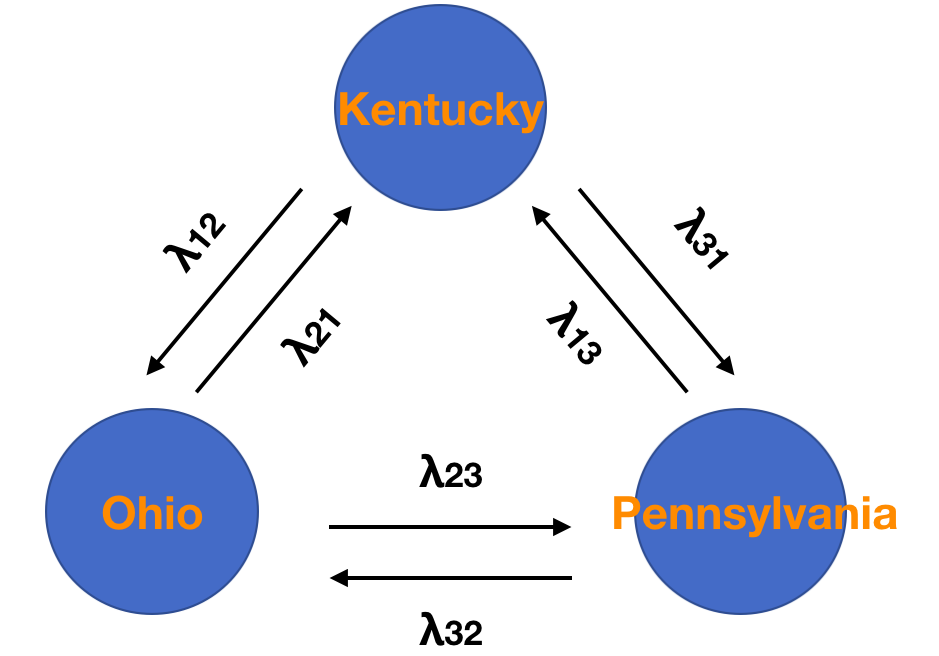
\includegraphics[width=10cm]{Fig/illustration}
\caption{Inter-state transmission}
\end{figure}

    \item Considering the internal spread of states (or counties), we hypothesized the growth radio within state (or county) $i$ is $\lambda{ii}$. Besides, we hypothesized that the attenuation radio within state (or county) $i$ is $\mu_i$.Therefore, like the previous section, we can establish following equations to describe the model:
$$
N_i[x_i(t+\Delta t) - x_i(t)] = \sum^5_{j=1}\lambda_{ji}N_jx_j(t)s_j(t)\Delta t - \mu_i N_ix_i(t)\Delta t \ \ \ \ \ \ ......(2.1)
$$
Then we added the initial conditions and establish the differential equation of the model:
$$
  \begin{cases} 
      \frac{dx(t)}{dt} = \sum^5_{j=1} \lambda_{ji}\frac{N_j}{N_i}x_j(t)s_i(t) - \mu_i x_i(t)  \\
      x_i(0) = x_{i_0}
  \end{cases}
, i = 1,2,3,4,5 \ \ \ \ \ \ ......(2.2)
$$
Similarly to the previous method, we established seven differential equations from \textit{MCM\_NFLIS\_Data}, and used least square method to get the approximate solution of $\lambda$ and $\mu$.Then, we got the model, which includes the spread of states (or counties). This time the fitness of our simulated curve is much better, which is analysed is section(3.4)
\end{enumerate}


\subsection{Result analysis}
Here attach the simulated result of our refined model described in section(3.3.2). Fig.8 corresponds to the spread among states and Fig.9 corresponds to the spread among counties.

In Fig.8, we select the spread of heroin as illustration. The blue curve is the simulated trend generated by our algorithm while the orange curve is the ground truth data points. For states $KY$, $OH$, $PA$ and $VA$ the simulated results are very close to the ground truth. For state $WV$, although the fitness is not quite good, the decreasing tendency can be obviously seen in the simulated curve, which can not be expressed by any other previous model we have tried.

\begin{figure}[!htbp]
\centering
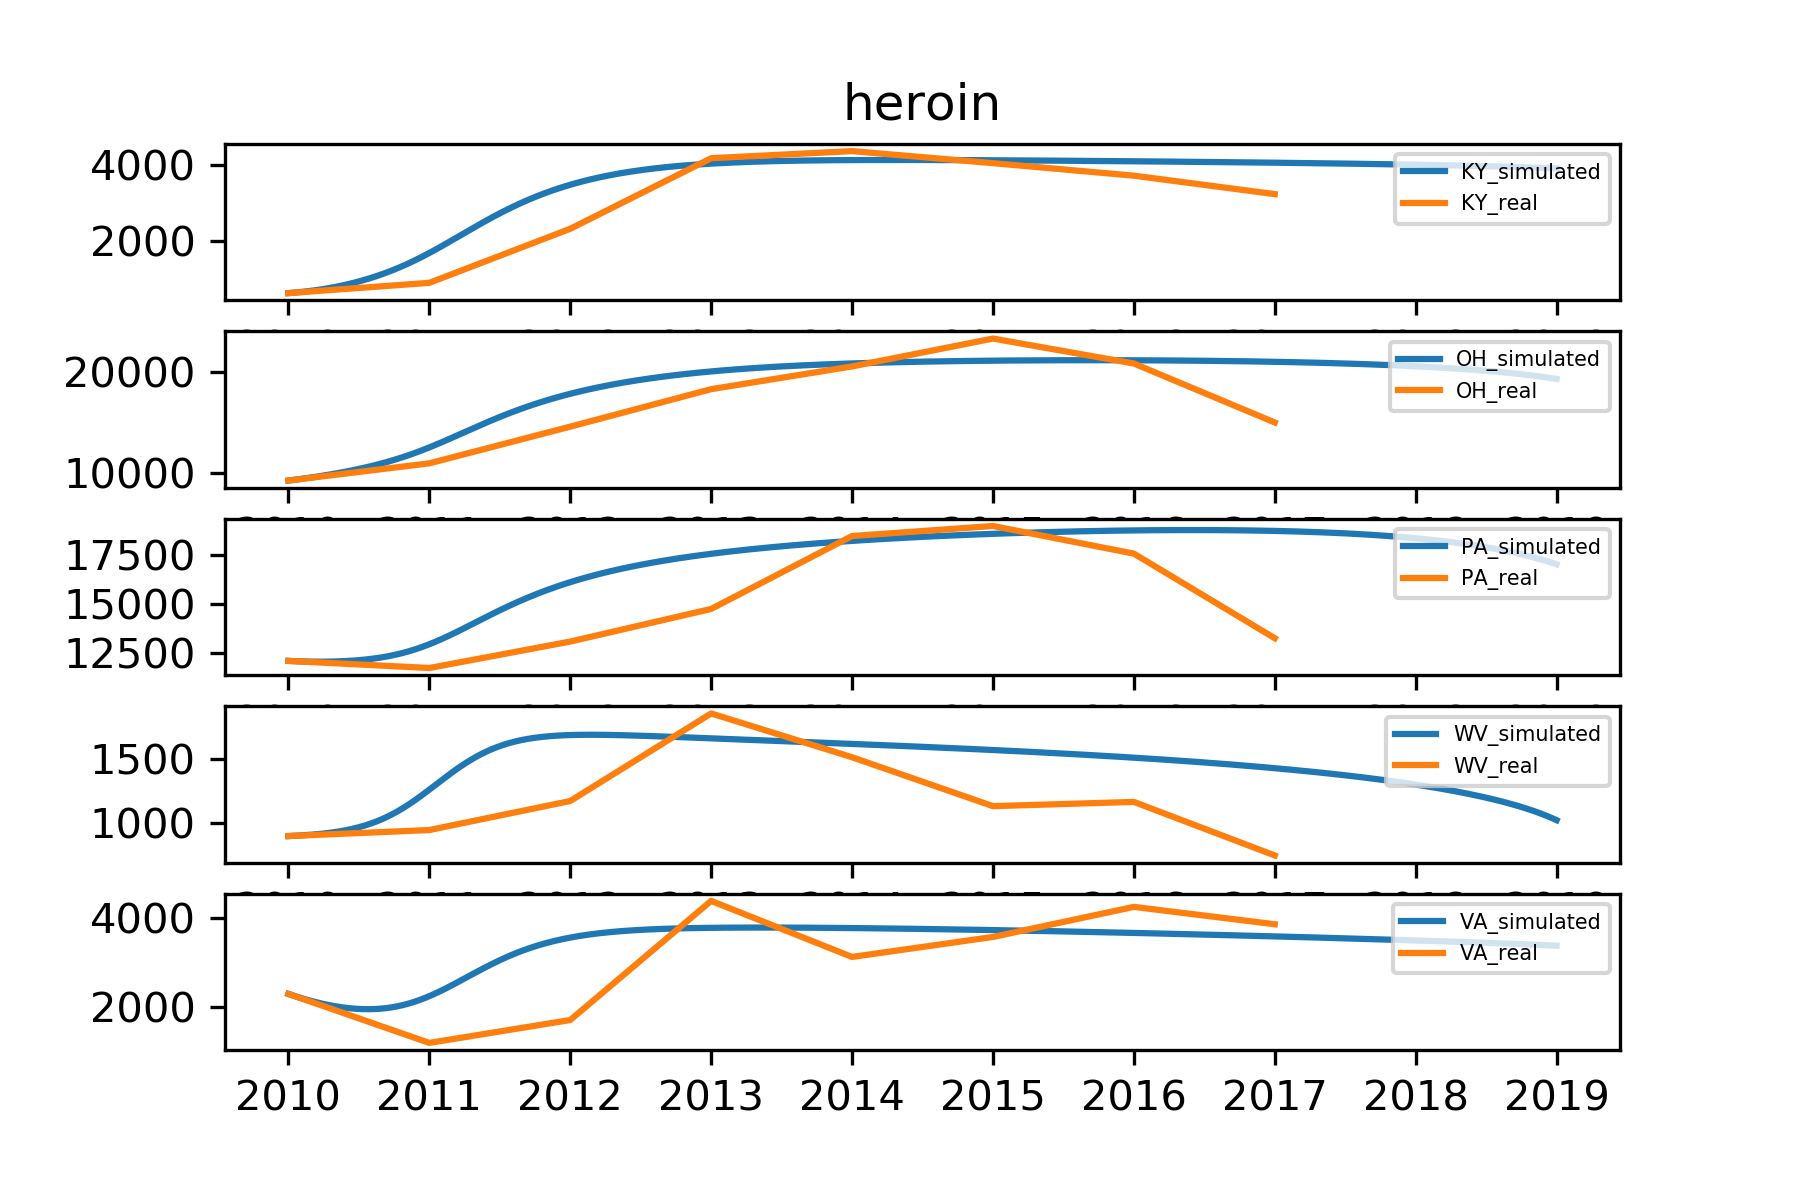
\includegraphics[width=16cm]{Fig/heroin_states_simul}
\caption{Heroin spread among states over time}
\end{figure}

In Fig.9, to illustrate, we select three typical substances: $Heroin$, $Fentanyl$, $Hydrocodone$. And for each typical substance, we select three counties. As we can see, the fitness of our simulated curve and the ground truth of $Fentanyl$ is fantastic and so do OH-HAMILTON with heroin, PA-LUZERNE with hydrocodone and KY-JEFFERSON with heroin.


\begin{figure}[!htbp]
\small
\centering
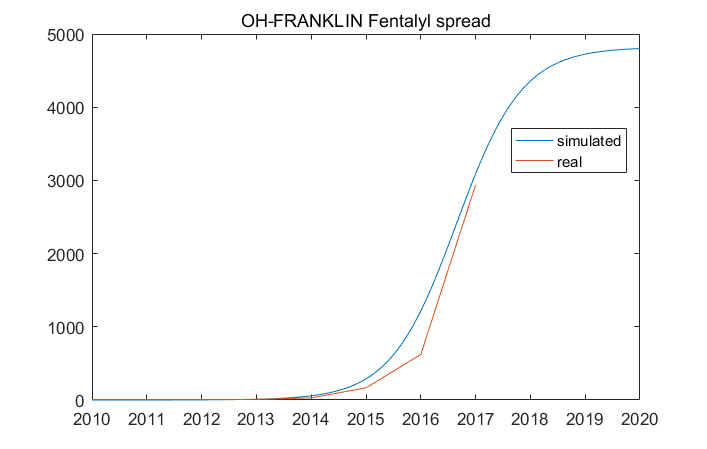
\includegraphics[width=5cm]{Fig/f1}
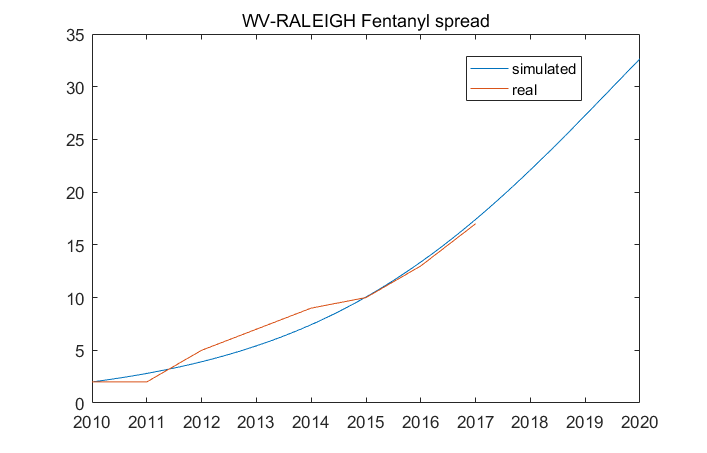
\includegraphics[width=5cm]{Fig/f2}
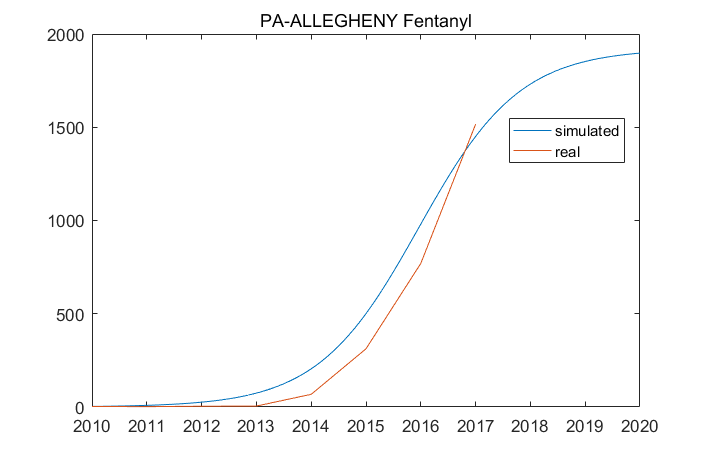
\includegraphics[width=5cm]{Fig/f3}
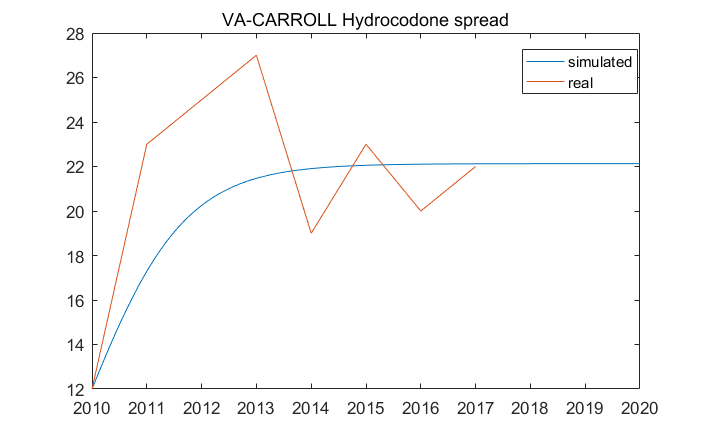
\includegraphics[width=5cm]{Fig/o1}
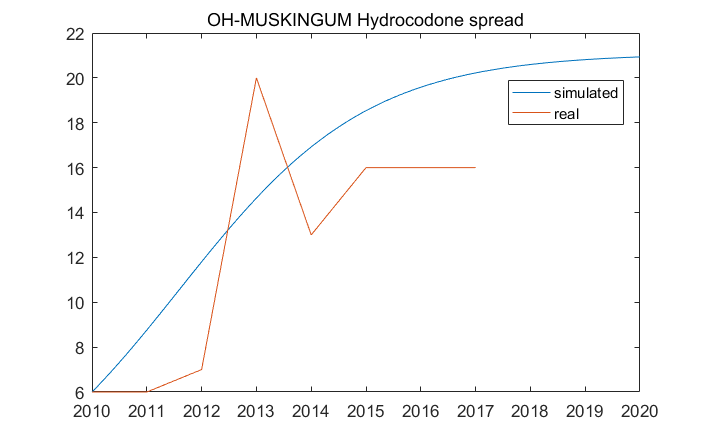
\includegraphics[width=5cm]{Fig/o2}
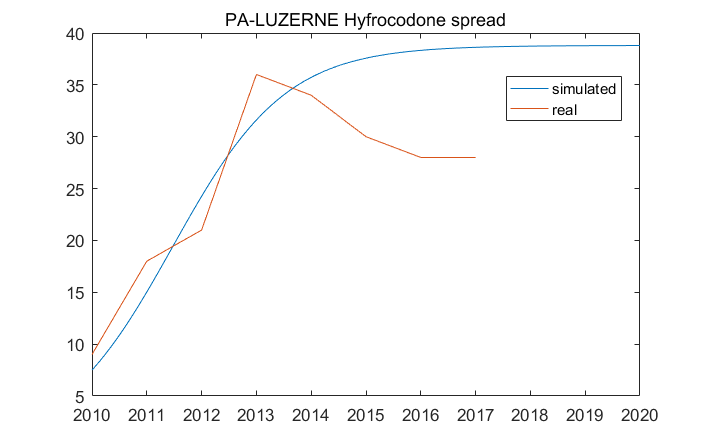
\includegraphics[width=5cm]{Fig/o3}
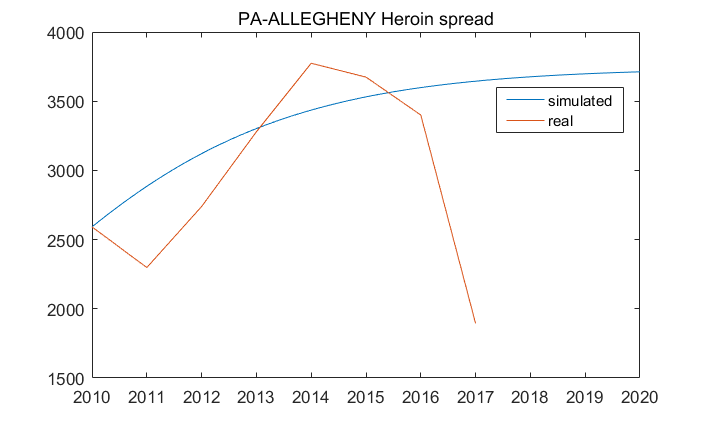
\includegraphics[width=5cm]{Fig/h1}
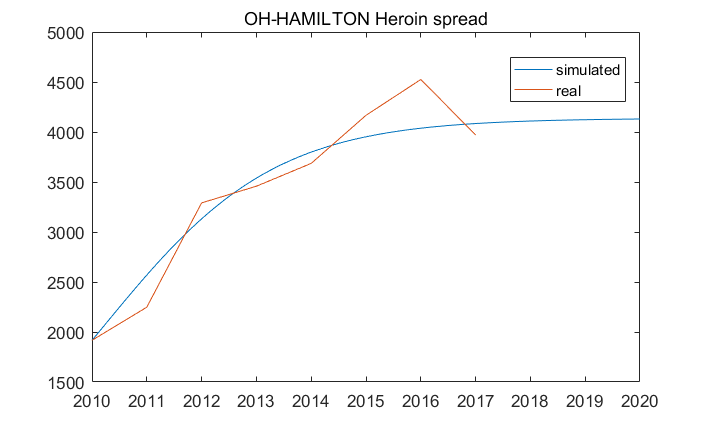
\includegraphics[width=5cm]{Fig/h2}
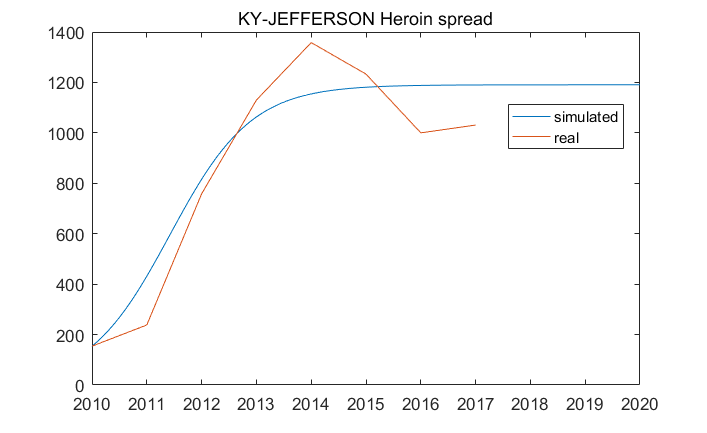
\includegraphics[width=5cm]{Fig/h3}
\caption{The spread of 3 typical substance among 3 selected counties}
\end{figure}


\subsubsection{Predictions and future concerns}
From the perspective of states, the use of heroin in state $KY$, $VA$ would still be at a high level in at least the following 2 years. The heroin level in state $OH$, $PA$, $WV$ would decrease gradually. The heroin in state $WV$ would be at a rather low level from 2018.

As for the cases among counties, an important fact that should be pay attention to is that the use of $Fentanyl$ is increasing at an astonishing rate. Both $Hydrocodone$ and $heroin$ fluctuate but still at a high rate. 

Refer to Fig.4[lower], the level of synthetic opioid except heroin arises in state $OH$, $PA$. Now we know that it should be owed to the growing use of $Fentanyl$, and 
$hydrocodone$ and maybe $oxycodone$ (though not presented in the figures). And for example, if cases of abusing $Fentanyl$ are reported, they are probably happened at least in FRANKLIN, RALEIGH, and ALLEGHENY in state $OH$.

%====================================================================
\section{Modified model}

\subsection{Additional notations}
Refer to Fig.10
\begin{figure}[!htbp]
\small
\centering
\includegraphics[width=16cm]{Fig/Additional_notations}
\caption{Additional notations}
\end{figure}

\subsection{Additional assumptions}

\begin{enumerate}[\bfseries 1.]

\item The factors within U.S. Census socio-economic data sheet are independent of each other.

\item The effects of various factors on the spread of opioids have only two states: perfect correlation or zero correlation.

\item The influence of various factors on the spread of opioid  can be compared, using the form of weights.

\item We ignore the impact of these factors on the spread of opioids between states and states.

\item We divide all the factors into two groups: internal factors and external factors. Internal factors derive from the growth and attenuation of drug cases described in our preliminary model while external factors denotes some new findings from U.S. census socio-economic data \textit{ACS\_xx\_5YR\_DP02} in this part.

\end{enumerate}

\subsection{Modeling}

\subsubsection{Factor selection}
 Give U.S. census socio-economic data \textit{ACS\_xx\_5YR\_DP02}, we try to find out several factors concerning the spread and the use of opioid. According to some social surveys and published papers, we select 9 possible factors over 209 given socio-economic factors: 
 \begin{enumerate}[\bfseries (1)]
     \item Married-couple family (with own children under 18 years)
     \item Male householder, no wife present, family (with own children under 18 years)
     \item Female householder, no husband present, family
     \item Householder living alone (65 years and over)
     \item Widowed
     \item Divorced
     \item Some college, no degree
     \item Bachelor's degree or higher (percent)
     \item Ancestry - West Indian (excluding Hispanic origin groups)
 \end{enumerate}
 For those 9 factors, we collect the corresponding data from 2010 to 2016 for each states and draw the following 9 figures (Fig.11), respectively.

\begin{figure}[!htbp]
\small
\centering
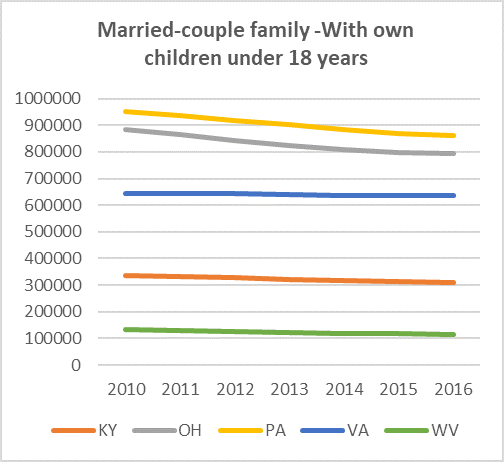
\includegraphics[width=5cm]{Fig/1}
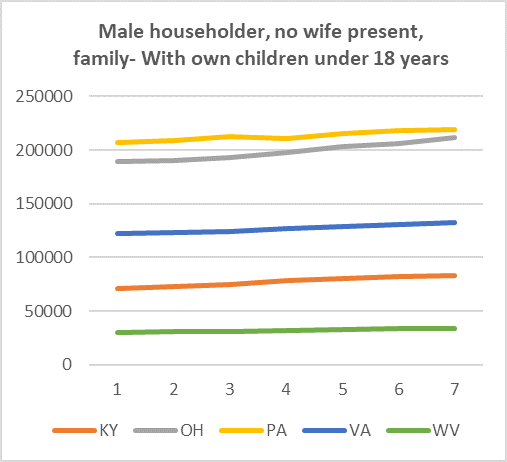
\includegraphics[width=5cm]{Fig/2}
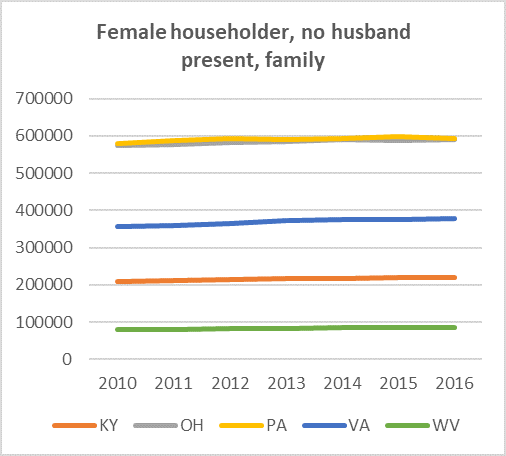
\includegraphics[width=5cm]{Fig/3}
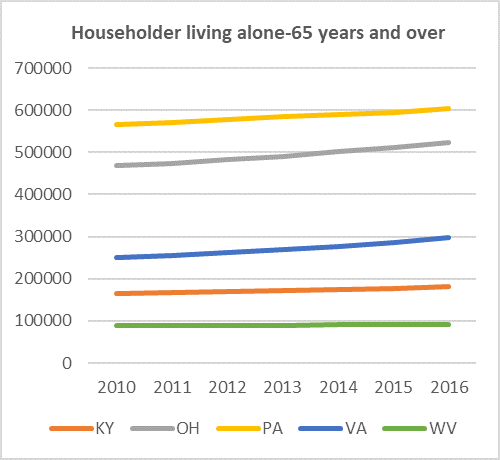
\includegraphics[width=5cm]{Fig/4}
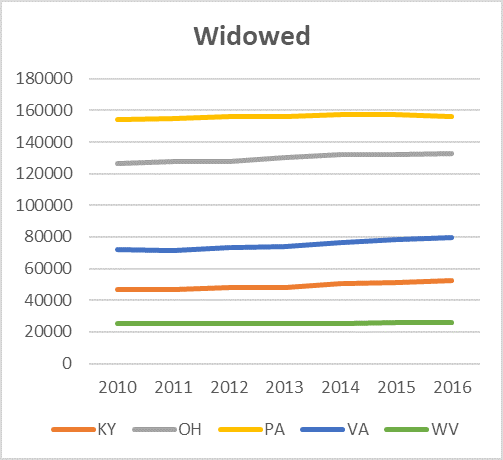
\includegraphics[width=5cm]{Fig/5}
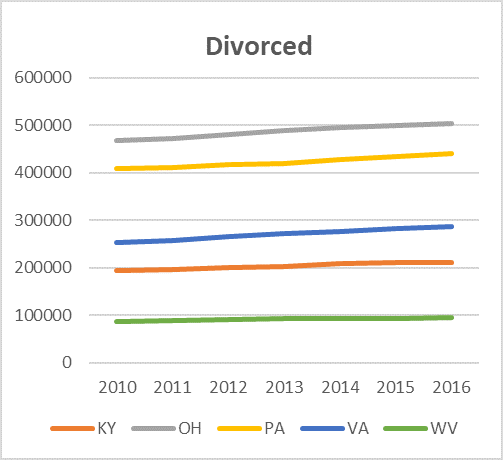
\includegraphics[width=5cm]{Fig/6}
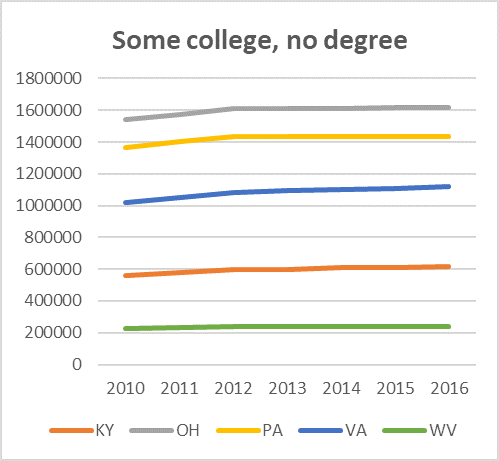
\includegraphics[width=5cm]{Fig/7}
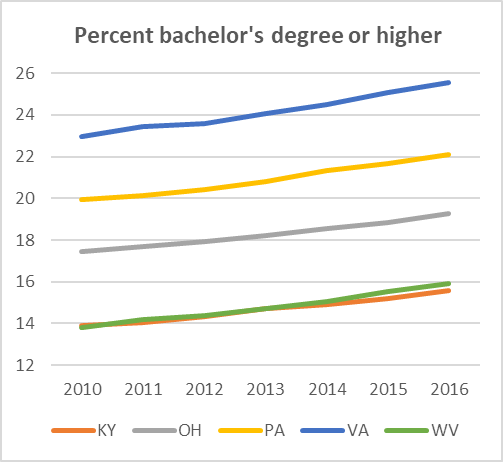
\includegraphics[width=5cm]{Fig/8}
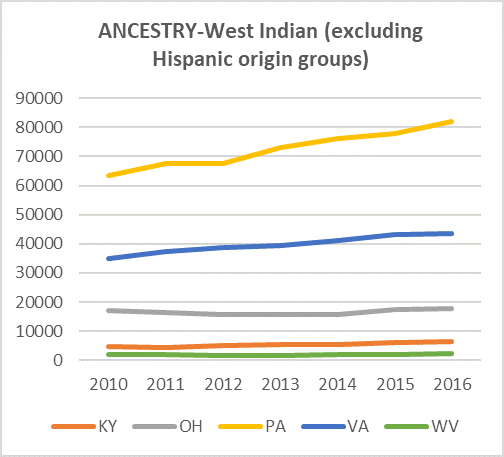
\includegraphics[width=5cm]{Fig/9}
\caption{9 possible factors in each states}
\end{figure}

Compared with the tendencies of spread of heroin and other synthetic opioid we got in Fig.4 in section(2). We choose 4 typical out of 9 possible factors above to modify our preliminary model illustrated in section(3):
 \begin{enumerate}[\bfseries (1)]
     \item Householder living alone (65 years and over)
     \item Divorced
     \item Ancestry - West Indian (excluding Hispanic origin groups)
     \item Bachelor's degree or higher (percent)
 \end{enumerate}
 
\subsubsection{Modifications on preliminary model}

First we apply Analytic Hierarchy Process (AHP) model$^{[3]}$ to calculate weights of those 4 factor. (AHP schema is illustrated as Fig.12)
\begin{figure}[!htbp]
\small
\centering
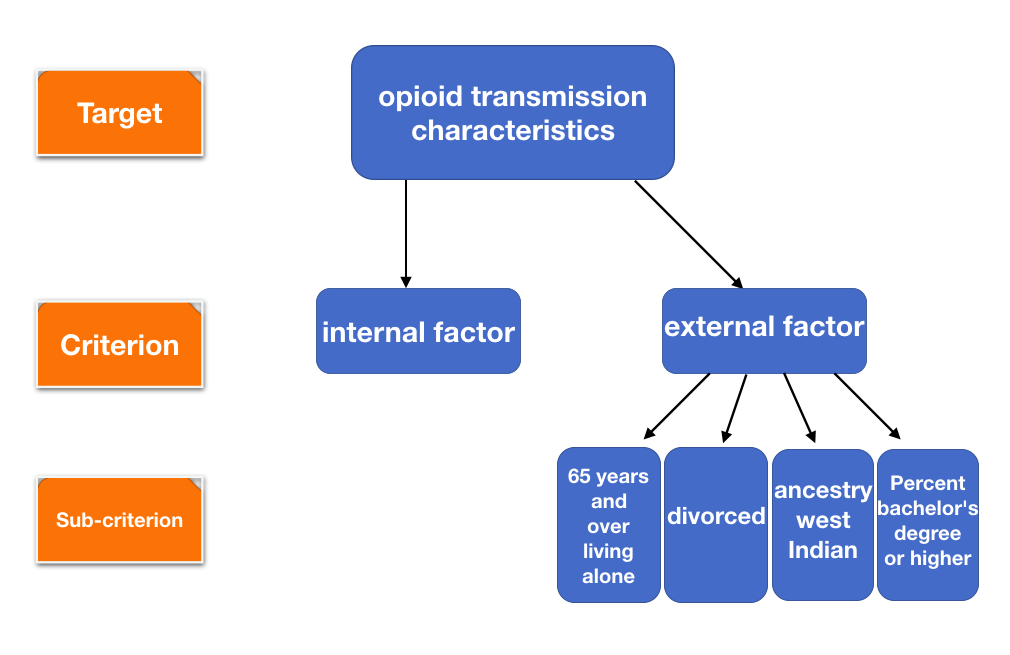
\includegraphics[width=14cm]{Fig/AHPmap}
\caption{AHP schematic diagram}
\end{figure}

Then we come up with the $R$ matrix (pair comparison judgement matrix), where $R_{ij}$ refers to a subjective grading of values varying from $1$ to $9$, published by \textit{Saaty}, which means how important factor $i$ is with respect to factor $j$. The more important factor $i$ is to factor $j$, the greater value $R_{ij}$ will be. Note that, by definition:
$$R_{ij} = 1 / R_{ji}, R_{ii} = 1$$
Here is the $R$ matrix for the criterion layer:
$$ R_{criterion} =
  \begin{pmatrix}
  {1} & {2}  \\
  {1/2} & {1}  \\
  \end{pmatrix}
$$
Considering the internal factor is 'level-2' important with respect to external factors, here we get $R_{12} = 2$. Then it is necessary to test the consistency of the R matrix. For $R_{criterion}$:
$$
a_{max}=2, CI=0, RI=0 \Rightarrow CR = 0 < 0.1
$$
check passes ($CR<0.1$ is the pass condition in AHP). The normalised eigenvector corresponding to the maximum eigenvalue $a_{max}$ is $[0.67, 0.33]$, i.e. the weight vector in the criterion layer is
$$ w_{criterion} =
  \begin{pmatrix}
  0.67  \\
  0.33  \\
  \end{pmatrix}
$$

Similarly, we apply the procedures above to the sub-criterion layer. According to U.S. census socio-economic data \textit{ACS\_xx\_5YR\_DP02}, we collect data corresponding to those 4 factors stated previously in section(4.3) and construct the $R$ matrix as follows:
$$ R_{sub\_criterion}
  \begin{pmatrix}
  {1} & {5} & {{1}/{2}}  & {{1}/{4}} \\
  {{1}/{5}} & {1} & {{1}/{6}}  & {{1}/{7}}\\
  {2} & {6} & {1}  & {{1}/{3}}\\
  {4} & {7} & {3}  & {1}\\
  \end{pmatrix}
$$
Check its consistency:
$$
a_{max} = 4.152, CI = \frac{4.152-4}{4-1}=0.051, RI=0.900 \Rightarrow CR = 0.056 < 0.1
$$ 
check passes. The normalised eigenvector corresponding to the maximum eigenvalue $a_{max}$ is $[0.159, 0.048, 0.249, 0.544]$, i.e. the weight vector in the criterion layer is
$$ w_{sub\_criterion} =
  \begin{pmatrix}
    0.159 \\
    0.048 \\
    0.249 \\
    0.544 \\
  \end{pmatrix} \Rightarrow
  w_{sub\_criterion\_global} = 0.33* w_{sub\_criterion}=
  \begin{pmatrix}
    0.053 \\
    0.016 \\
    0.083 \\
    0.181 \\
  \end{pmatrix}
$$
where $w_{sub\_criterion\_global}$ ($w$, for short, in the rest of this paper) is the weight vector for external factors from the perspective of criterion layer.

By observation on Fig.11, we find those factors basically change linearly over time.  All the linear slopes are shown in Fig.13 (calculate from Fig.11). Note that the number of people who get bachelor's degree or higher actually increases. But it is reported that the better a person gets educated, the less possibly he will abuse drugs so we set the fourth column of Fig.13 negative values. We also assume that those factors linearly influence the spread of drug. Here for state $i$ we derive the influence vector $k_i$ coming from row-i of Fig.13. For example, 
$$
k_{KY} = [0.0151, 0.0154, 0.0563, -0.0285]^T
$$
Counting in such influence, we modify $x_i(t)$ in equation(2.2),
$$
x_i(t) \leftarrow 0.67x_i(t) + 0.33 (w\cdot k_{KY})t
$$
\begin{figure}[!htbp]
\small
\centering
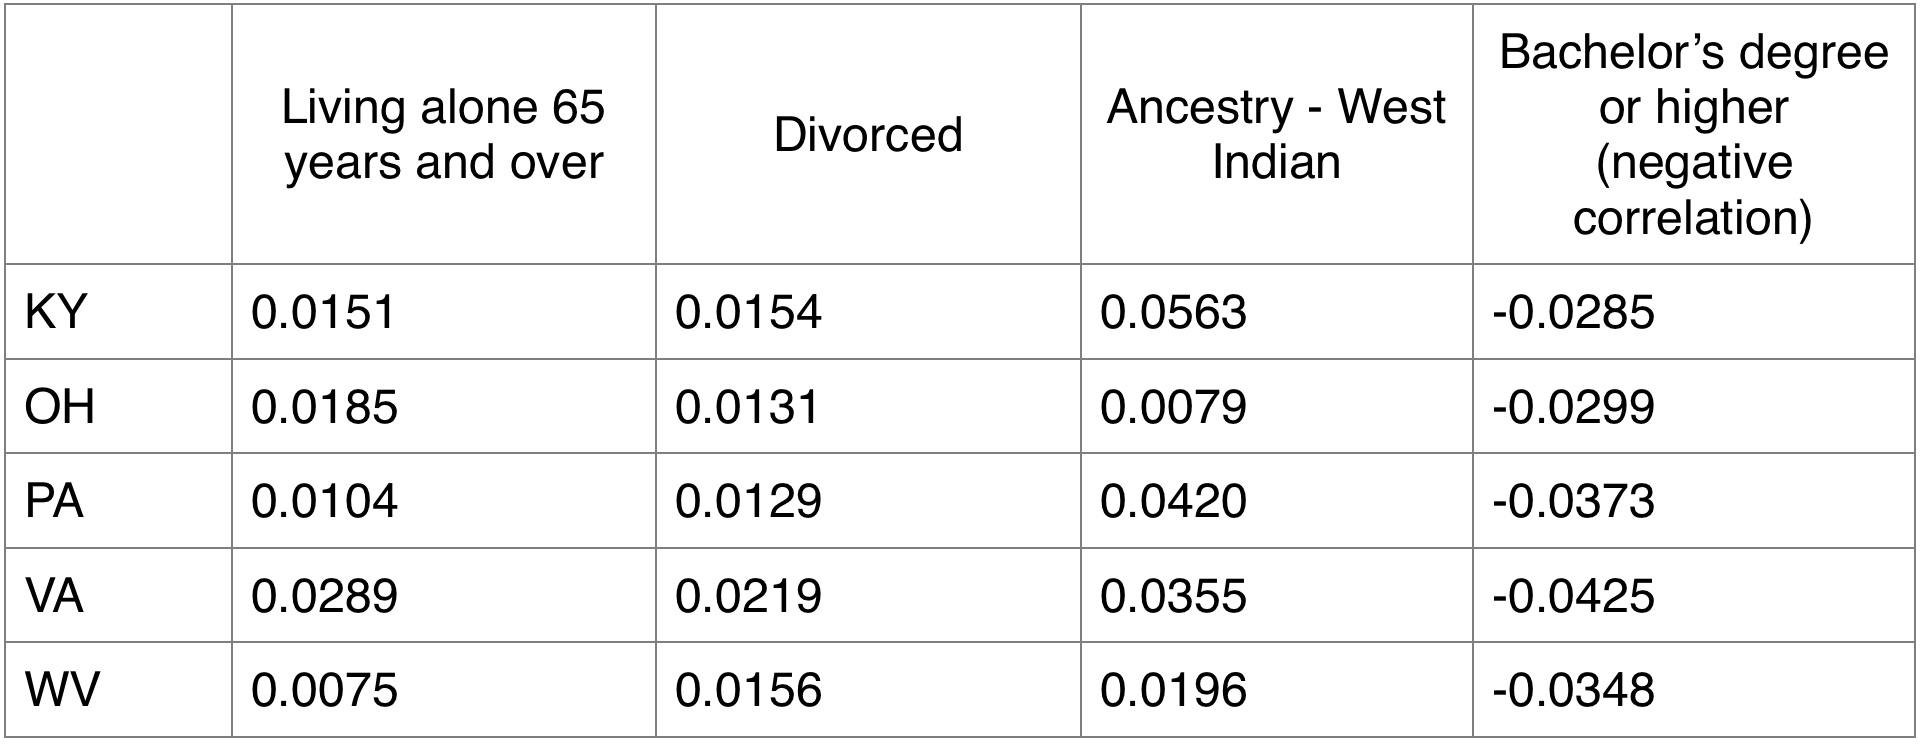
\includegraphics[width=16cm]{Fig/k_states}
\caption{Slopes of each factor in each state}
\end{figure}

\subsection{Result analysis}
This time we still choose heroin incidents as an example for illustration. Here attach the simulated results (Fig.14[lower]) with the previous results (Fig.14[upper]). Compared with the preliminary model, it can be obviously seen that the simulated curves generated by the modified model fit much better with the ground truth.

And the problem is that the number of heroin incidents of some states, like $PA$ and $WV$, drops quickly after 2015-2016, which is still not presented in this modified model since we did not take the interference from government into consideration. And this issue would be fixed by the strategies we come up with in section(5).

\begin{figure}[!htbp]
\small
\centering
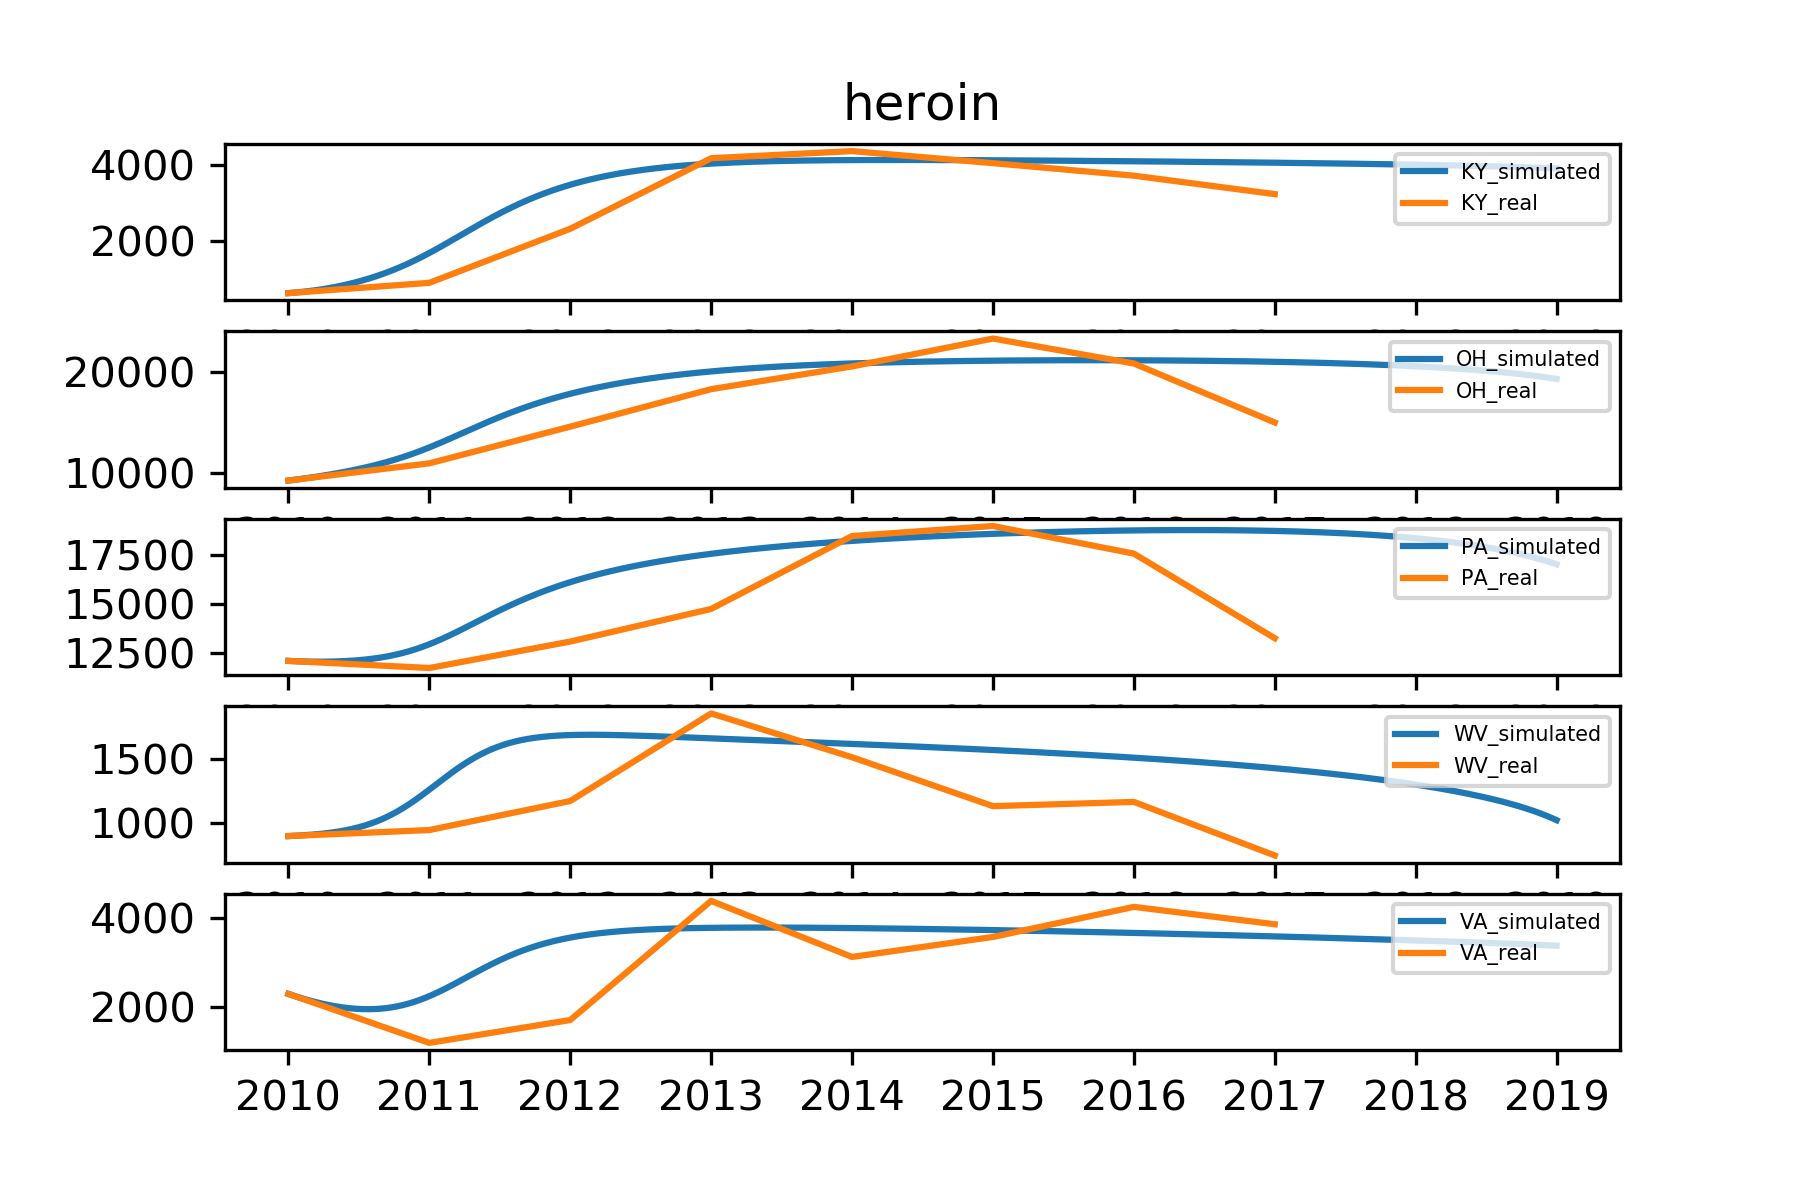
\includegraphics[width=16cm]{Fig/heroin_states_simul.png}
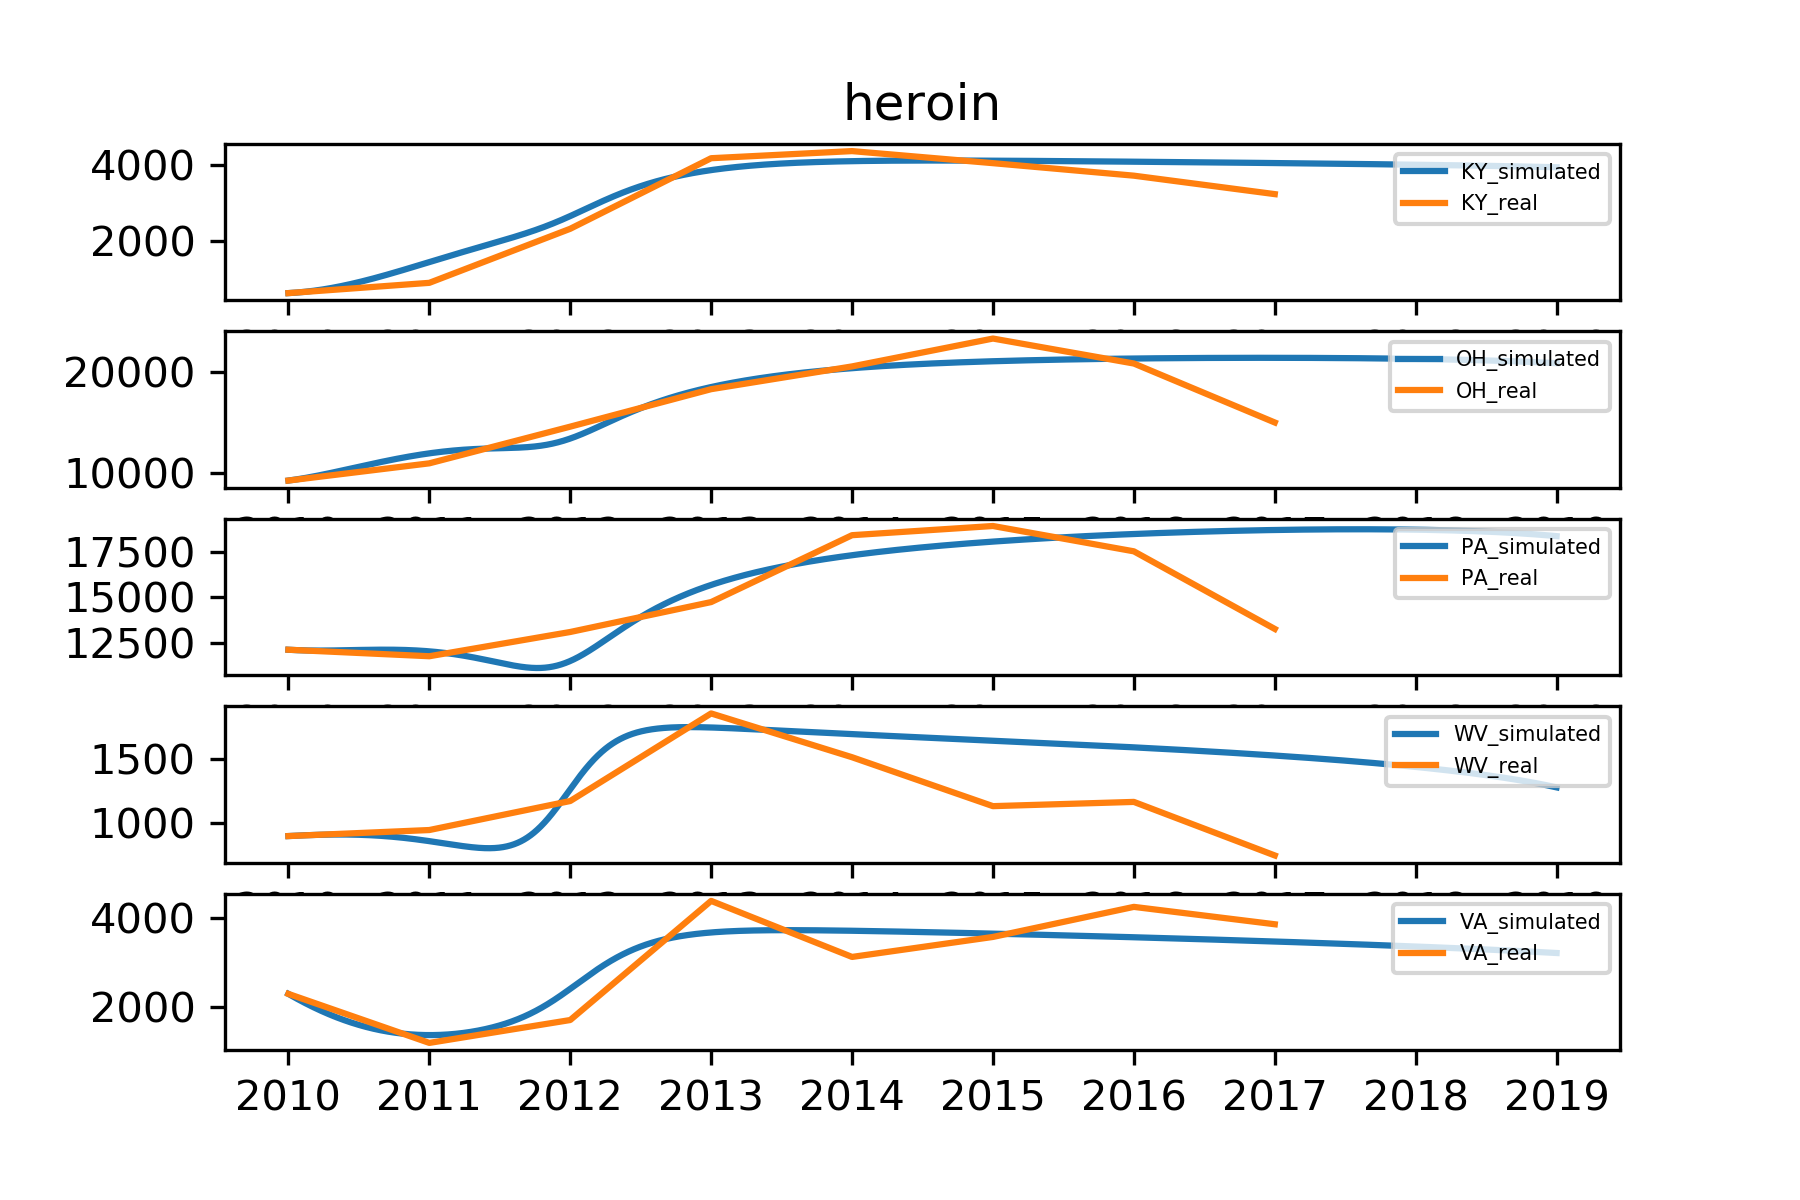
\includegraphics[width=16cm]{Fig/heroin_states_simul_modified.png}
\caption{Preliminary model (upper) and modified model (lower)}
\end{figure}

\section{Strategies}
According to the combination of  Part 1 and Part 2 results, the opioid crisis has eased a bit, since the US government began to take corresponding measures. However, the use of fentanyl doesn't decrease, and the number of divorced and low-educated families is positively correlated with the use of opioids. Based on this, we suspected that the current strategy is lacking in the three aspects of mentality factor, media report and relevant system. We came up with a possible strategy (Fig.15) including 5 parts: 
\begin{enumerate}[\bfseries (1)]
    \item Use psychological counseling to reduce the patient's attention on pain. 
    \item Advocating a philosophy of the similar type of Taoism to ease the impetuous atmosphere 
    \item Use the media to correct wrong opinions, such as: opioids have low addiction 
    \item Improve the standard of rational opioid use
    \item Fight against the black market, and reduce the reimbursement ratio of opioids.
 \end{enumerate}

\begin{figure}[!htbp]
\small
\centering
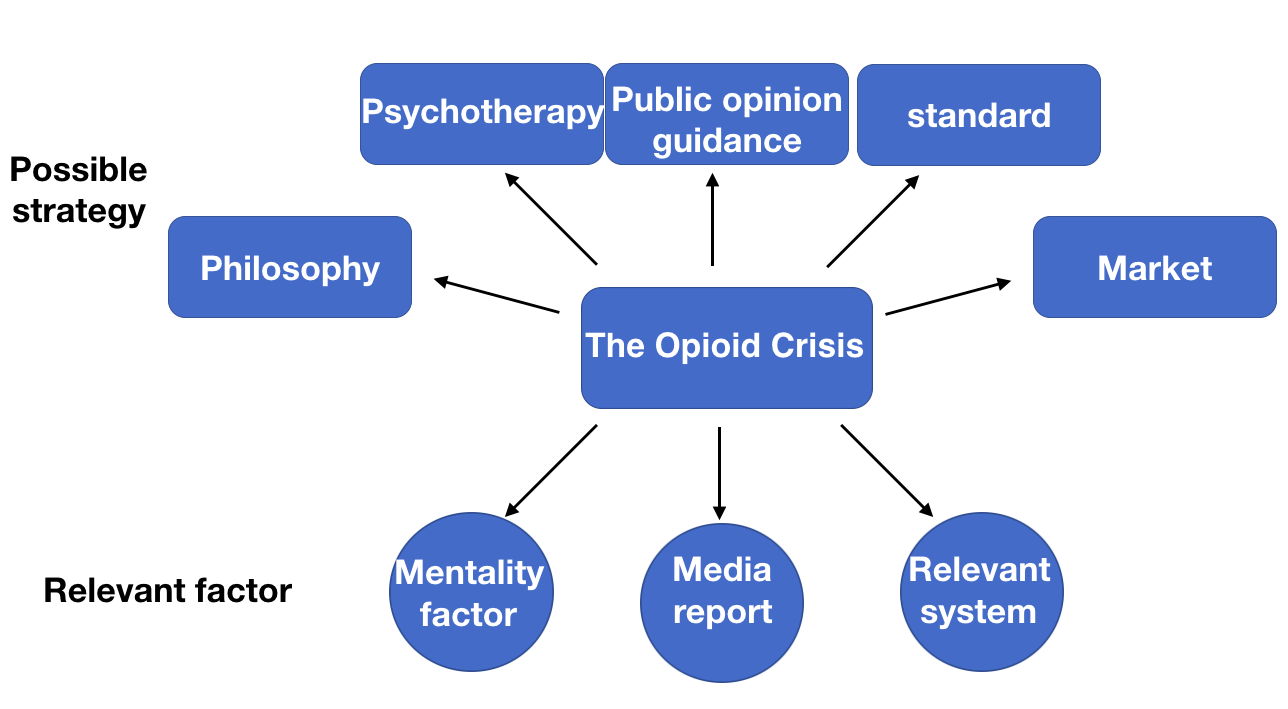
\includegraphics[width=12cm]{Fig/str.png}
\caption{Strategies}
\end{figure}

\subsection{Stablities}
The influence of these strategies on the parameters of the model is reflected in the internal factor spread rate $\lambda_{ij}$ and the external factor spread rate $k$. It can reduce the values of $\lambda_{ij}$ and $k$ at the same time. By adjusting the values of $\lambda_{ij}$ and $k$ in the model, we can see the effect of these strategies on the trend of opioid transmission. We take the spread of heroin in Kentucky as an example (shown in Fig.16):

\begin{figure}[!htbp]
\small
\centering
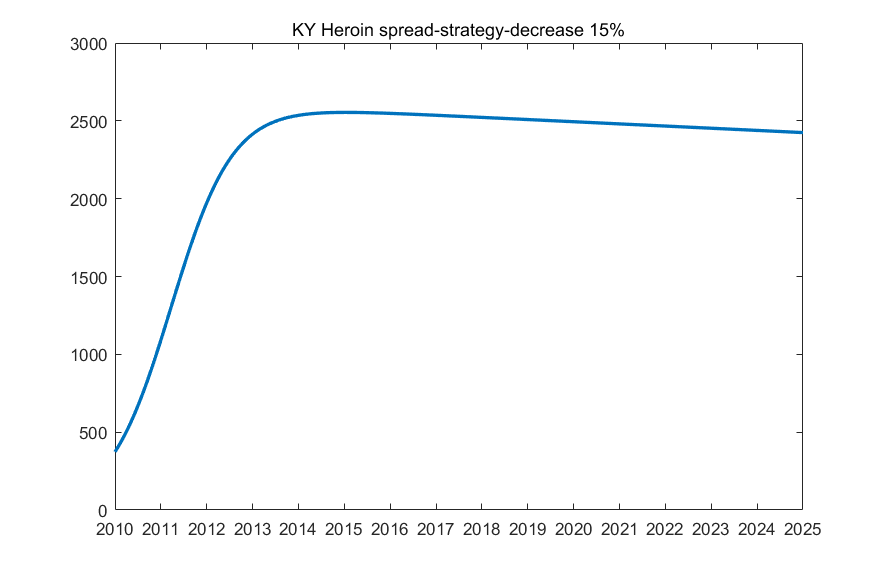
\includegraphics[width=7cm]{Fig/15_percent.png}
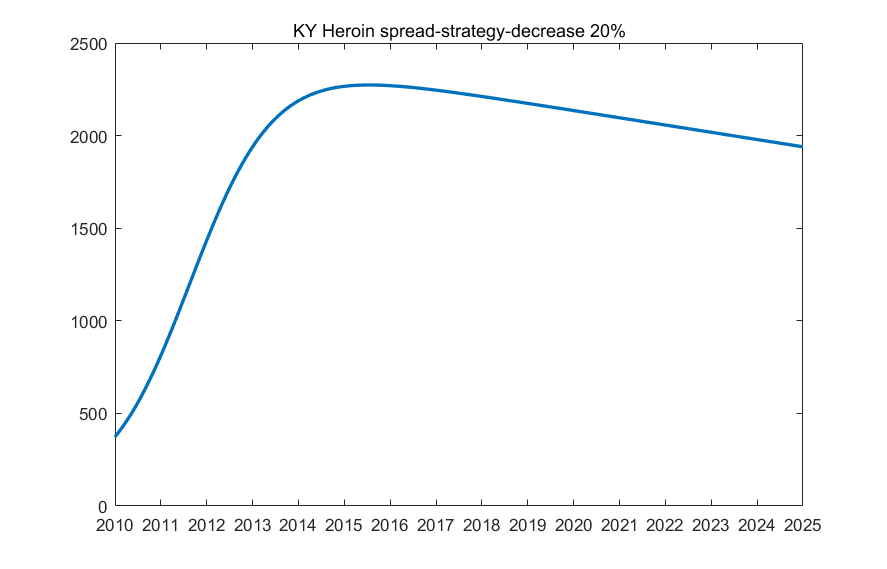
\includegraphics[width=7cm]{Fig/20_percent.png}
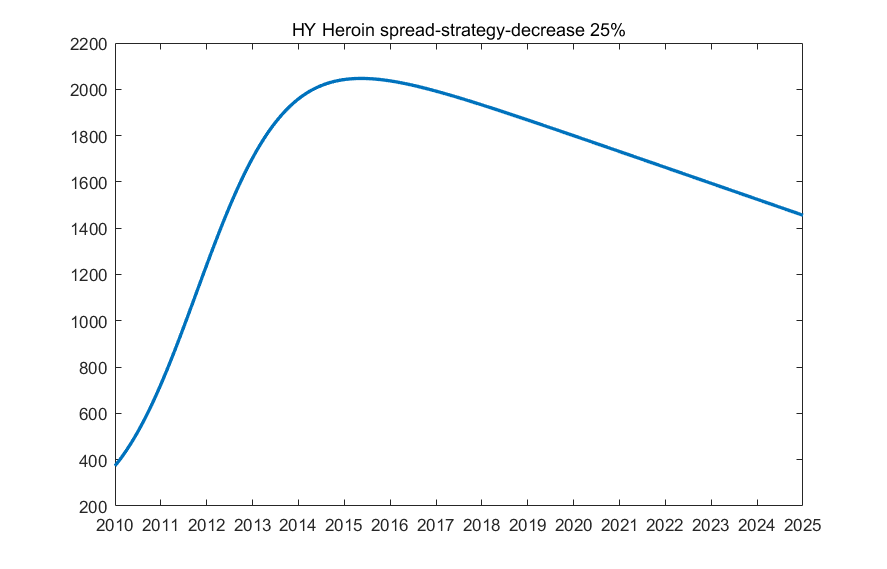
\includegraphics[width=7cm]{Fig/25_percent.png}
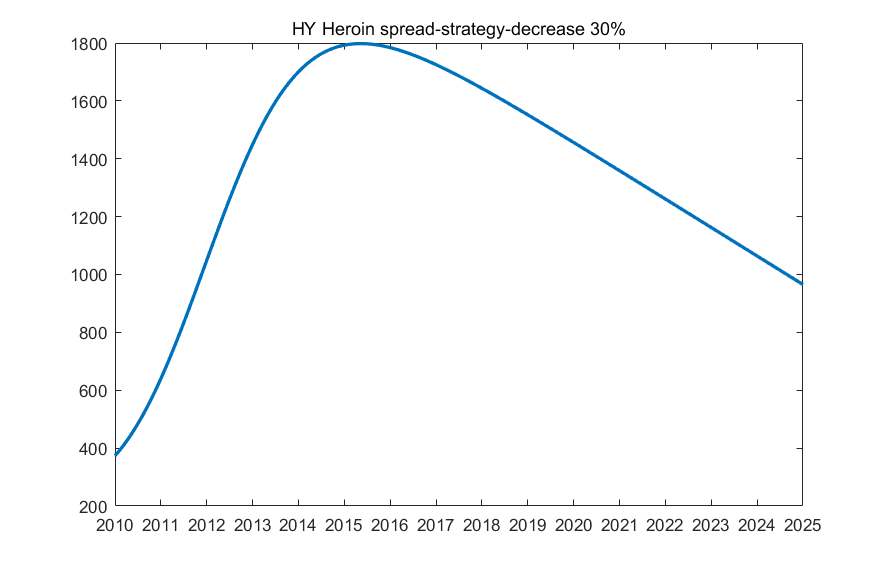
\includegraphics[width=7cm]{Fig/30_percent.png}
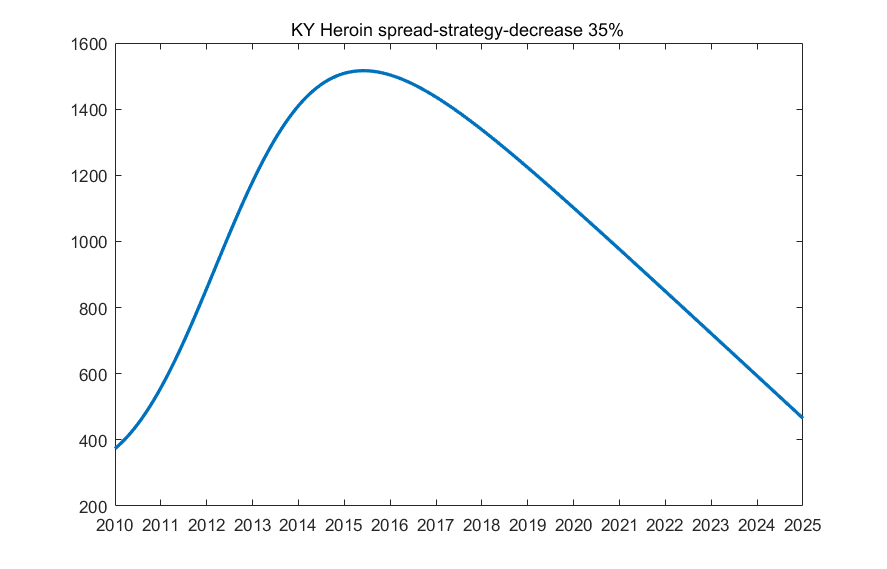
\includegraphics[width=7cm]{Fig/35_percent.png}
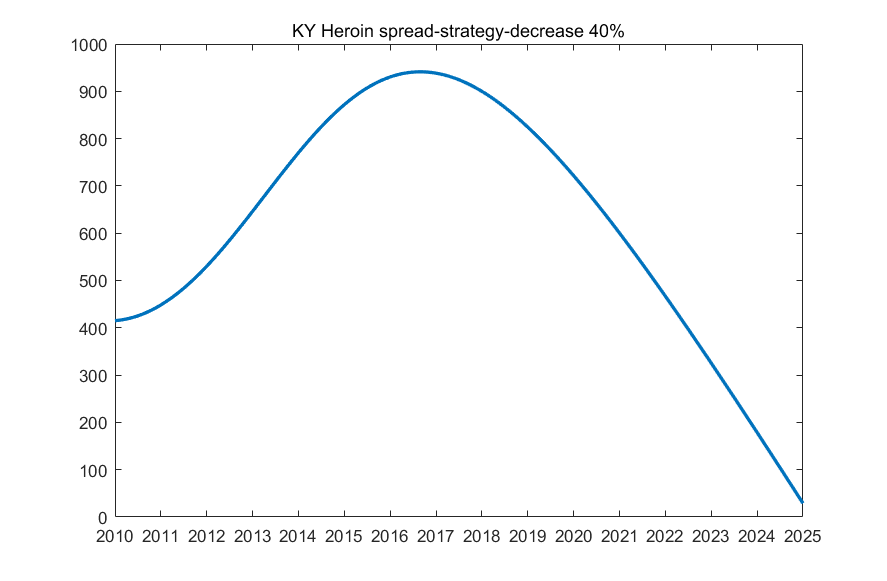
\includegraphics[width=7cm]{Fig/40_percent.png}
\caption{Influence of strategies at different level}
\end{figure}

After several attempts, we found that only if the value of $\lambda_{ij}$ and $k$ are reduced by at least $20\%$ can it help curb the continued growth and spread of opioids. In other words, our strategy to control opioids is realized by at least a $20\%$ reduction in overall spreading.

\section{Strengths and Weaknesses}
\subsection{Strengths}
 \begin{enumerate}[\bfseries (1)]
    \item We leave out irrelevant variables, making the model simple and concise.
    \item By making schematics and figures, we make the model more clear and more applicable.
    \item Our model is easy to add more influencing factors in the future, which may facilitate the upgrade of the model.
    \item We analyzed the opioids separately, better distinguishing the differences between the opioids, and finding the specific transmission characteristics of certain opioid (such as fentanyl).
 \end{enumerate}

\subsection{Weaknesses}
\begin{enumerate}[\bfseries (1)]
\item The threshold, estimated from known data trends for opioid spread, may exist a little bit large errors.
\item We are less concerned about social and economic factors, which may lead to errors in the prediction results.
\item The analytic hierarchy process, which is used in determining the weights, contains certain subjective judgment.
\item The fitting of the model is not very well when there exists large fluctuation to the data.
\end{enumerate}

\section*{Acknowledgement}
During this project, we collaborate within a group of three members \textit{Zengpeng Li}, \textit{Fengming Zhu} and \textit{Manding Wang}. Great thanks to \textit{Prof. Zhongkai Liu}.


%\begin{thebibliography}{99}
%\addcontentsline{toc}{section}{References}  %引用部分标题("Refenrence")的重命名
%\bibitem{1}Elisa T. Lee, Oscar T. Survival Analysis in Public Health Research. \emph{Go. College of Public Health}, 1997(18):105-134.
%\bibitem{2}Wikipedia: Proportional hazards model. 2017.11.26. \texttt{\\https://en.wikipedia.org/wiki/Proportional\_{}hazards\_{}model}
%\end{thebibliography}
\pagebreak
\section{Memo}
Dear Sir or Madame,

Based on the data provided, we establish a customized model to develop accurate projections and try to come up with strategies to control the spread of opioids around those five states.

Firstly, We apply SIS model to predict the trend of opioids detection rate in a certain state over time, regardless of external factors. Furthermore, counting in some exogenous factors from socio-economy data sheet, we get 4 main influencing factors. And then we use Analytic Hierarchy Process (AHP) to get the weight of the 4 factors. Finally we simulate our modified model, whose results fit well in the ground. 

Through the established model, we got a lot of information and discoveries. The significant insights and results we identified are:
\begin{enumerate}[\bfseries (1)]
\item The spread of opioids generally showed a trend of rising first and then decreasing a little. We believe that the decline was mainly affected by government regulation.
\item Older people who are living alone and divorced people are more inclined to use opioids and should be given special attention.
\item Increasing people’s education can significantly reduce the use of opioids.
\item The speed of fentanyl is extremely fast and requires special attention.
\end{enumerate}


Building upon our model, detecting the use of $fentanyl$ is very important. 
Fentanyl is a synthetic opioid for pain reliever which is 50 to 100 times more potent than morphine. Because of its stronger efficacy and low price, its usage is increasing year by year. In view of this situation, we suggest:

\begin{figure}[!htbp]
\small
\centering
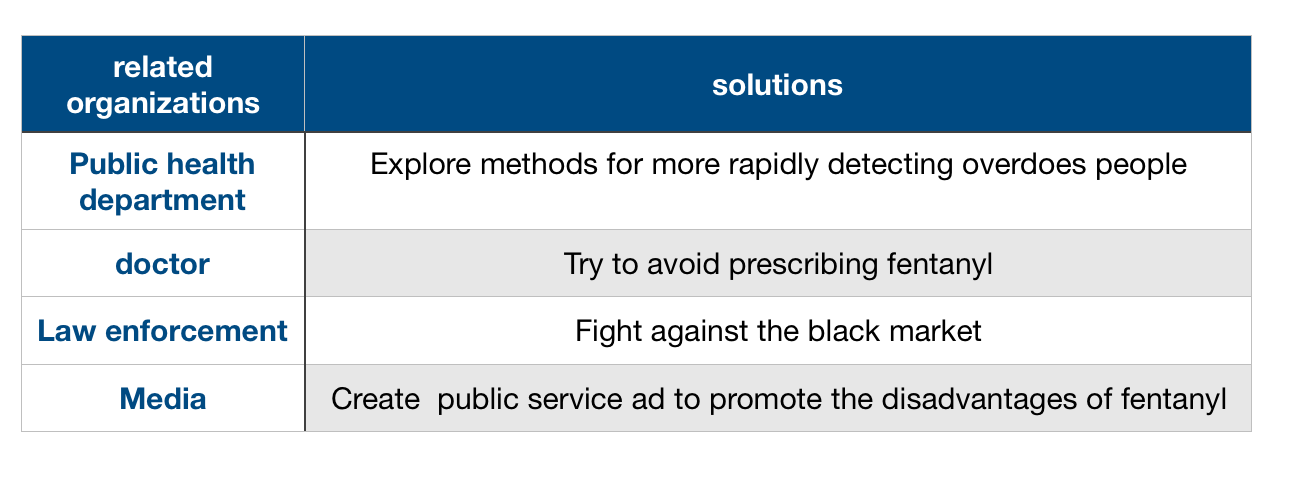
\includegraphics[width=16cm]{Fig/memo1.png}
\caption{Strategies for Fentanyl incidents}
\end{figure}

Divorces and non-graduates, who are not rational enough, are easier to take opioids. So detecting use of opioids of divorces and non-graduates is very important. In view of this situation, we suggest:

\begin{figure}[!htbp]
\small
\centering
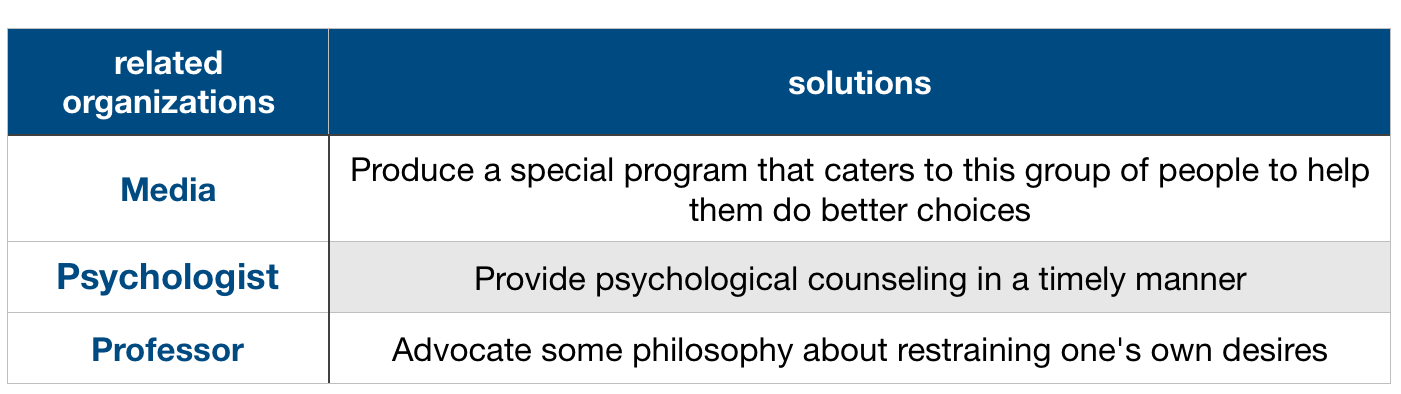
\includegraphics[width=16cm]{Fig/memo2.png}
\caption{Strategies for divorces and non-graduates}
\end{figure}

This is a long process to resolve the crisis, but we believe that using mathematical modeling methods to predict and analyze and launching the whole society to face and solve this problem will make things better and better.\\


Sincerely,

Team\# 1916056

\pagebreak
\section{References}
[1] "Mathematical Modeling", Kuishou Si, Xijing Sun, National Defense Industry Press, 2017.4 

[2] "The research of analysis and application of SIS Epidemic model",\\
https://www.docin.com/p-844931483.html

[3] "Research on Entropy Weight-AHP and Grey-Analytic Hierarchy Process", Zhicong Fei, 2009.5

[4] "The Opioid Crisis", Mahan, Kieran T, The Journal of Foot and Ankle Surgery, January-February 2017, Vol.56(1), pp.1-2 

% ==============以下为附录内容,如您的论文中不需要程序附录请自行删除====================
\clearpage
\begin{subappendices}						% 附录环境
\section*{Apendix: The source codes}		% 附录标题可以自行修改
\addcontentsline{toc}{section}{Appendix}  	% 将附录内容加入到目录中

This python program is used to simulate our model, the main part of the program is shown below.
\begin{lstlisting}[language=python, caption=\texttt{modeling.py}]
import pandas as pd
import numpy as np
import matplotlib.pyplot as plt
from scipy.integrate import odeint
# N table
N_table = [[0 for j in range(5)] for i in range(8)]
for i in range(8): 
    for j in range(5):
        N_table[i][j] = (N[j] - heroin_table[i][j])/N[j]
N_table = np.mat(N_table)
print(N)
print(N_table)

for city_index in range(table_header.shape[0]):
    A = np.mat(np.zeros([6,6]))
    for i in range(5):
        A[:,i] = np.multiply(np.mat(heroin_table[:6,i]).T, N_table[:6,city_index])
    A[:,5] = np.mat(heroin_table[:6,city_index]).T
#     print(A)
    b = np.mat(heroin_delta_table[:6,city_index]).T
#     print(b)
    x = (A.T.dot(A)).I.dot(A.T.dot(b))
#     print(x)
    for lam in range(5):
        Lambda[lam][city_index] = float(x[lam])
    Mu[city_index] = float(x[5])
    
def equations(y, t, Lambda, Mu):
#     Lambda, Mu = args
    ret = np.zeros(5)
    for col in range(5):
        for row in range(5):
            ret[col] += Lambda[row][col]*y[row]*(1-y[col])*N[row]/N[col]
        ret[col] += Mu[col]*y[col]
    return ret
y0 = [heroin_table[0][i]/float(N[i]) for i in range(5)]
# print(y0)
t = np.linspace(0,9,10001)
sol = odeint(equations, y0, t, args=(Lambda,Mu))
# print(sol)
# print(heroin_table)
# print(N)
for i in range(5):
    plt.subplot(5,1,i+1)
    plt.plot(t, sol[:,i]*N[i], label=(table_header[i].upper()+'_simulated'))
    plt.plot([j for j in range(8)], [heroin_table[j,i] for j in range(8)],\
     label=(table_header[i].upper()+'_real'))
#     plt.yticks([x for x in range(10000)])
    plt.xticks([x for x in range(10)], [str(i) for i in range(2010,2020)])
    plt.legend(loc=1, fontsize=5)
    if i == 0:
        plt.title('heroin')
\end{lstlisting}




\end{subappendices}
% =================================================================================



\end{document}